\documentclass[11pt,a4paper]{article}

% --- Core Geometry and Page Setup ---
\usepackage[margin=1in,headheight=14pt]{geometry}
\usepackage[utf8]{inputenc}
\usepackage[T1]{fontenc}
\usepackage{lmodern}
\usepackage{microtype}

% --- Mathematics and Symbols ---
\usepackage{amsmath,amssymb,amsthm}

% --- Color Palette and Graphics ---
\usepackage[table,xcdraw]{xcolor}
\usepackage{graphicx}
\usepackage{float}
\usepackage{tikz}
\usetikzlibrary{shapes.geometric,arrows.meta,positioning,calc,fit,backgrounds,shadows.blur}

% --- Tables and Arrays ---
\usepackage{booktabs}
\usepackage{tabularx}
\usepackage{array}
\usepackage{longtable}
\usepackage{colortbl}
\newcolumntype{L}[1]{>{\raggedright\arraybackslash}p{#1}}
\newcolumntype{Y}{>{\raggedright\arraybackslash}X}

% --- Lists and Compaction ---
\usepackage{enumitem}
\setlist[itemize]{nosep, leftmargin=*, topsep=2pt, partopsep=0pt}
\setlist[enumerate]{nosep, leftmargin=*, topsep=2pt, partopsep=0pt}

% --- Header, Footer, and Pagination ---
\usepackage{fancyhdr}
\usepackage{lastpage}
\pagestyle{fancy}
\fancyhf{}
\fancyhead[L]{\footnotesize\textbf{CSE 0613-3109:} System Analysis \& Design}
\fancyhead[R]{\footnotesize\nouppercase{\leftmark}}
\fancyfoot[L]{\small Khwaja Yunus Ali University (KYAU) --- Department of CSE}
\fancyfoot[R]{\small Page \thepage\ of \pageref{LastPage}}
\renewcommand{\headrulewidth}{0.5pt}
\renewcommand{\footrulewidth}{0.5pt}

% --- Typography and Section Titles ---
\usepackage{titlesec}
\titleformat{\section}
  {\normalfont\Large\bfseries\color{primaryNavy}}{\thesection}{1em}{}[\color{primaryNavy}\titlerule]
\titleformat{\subsection}
  {\normalfont\large\bfseries\color{secondaryBlue}}{\thesubsection}{1em}{}
\titleformat{\subsubsection}
  {\normalfont\normalsize\bfseries\color{slateGray}}{\thesubsubsection}{1em}{}

% --- Penalties to Prevent Widows and Orphans ---
\widowpenalty=10000
\clubpenalty=10000
\brokenpenalty=10000
\predisplaypenalty=10000

% --- Color Definitions ---
\definecolor{primaryNavy}{RGB}{20, 45, 85}
\definecolor{secondaryBlue}{RGB}{35, 95, 160}
\definecolor{slateGray}{RGB}{60, 75, 95}
\definecolor{lightBg}{RGB}{248, 250, 253}
\definecolor{tableHeader}{RGB}{232, 240, 250}
\definecolor{boxBorder}{RGB}{180, 205, 230}
\definecolor{caseBorder}{RGB}{210, 130, 40}
\definecolor{caseBg}{RGB}{254, 251, 246}
\definecolor{auditBorder}{RGB}{40, 140, 100}
\definecolor{auditBg}{RGB}{246, 253, 249}

% --- tcolorbox Callout Environments ---
\usepackage[most]{tcolorbox}
\newtcolorbox{conceptcard}[1]{
  colback=lightBg,
  colframe=secondaryBlue,
  coltitle=white,
  fonttitle=\bfseries\small,
  title={#1},
  arc=3pt,
  boxrule=0.8pt,
  left=8pt, right=8pt, top=6pt, bottom=6pt,
  before skip=8pt, after skip=8pt
}

\newtcolorbox{casestudybox}[1]{
  colback=caseBg,
  colframe=caseBorder,
  coltitle=white,
  fonttitle=\bfseries\small,
  title={Applied Case Study Analysis: #1},
  arc=3pt,
  boxrule=0.8pt,
  left=8pt, right=8pt, top=6pt, bottom=6pt,
  before skip=8pt, after skip=8pt
}

\newtcolorbox{governancebox}[1]{
  colback=auditBg,
  colframe=auditBorder,
  coltitle=white,
  fonttitle=\bfseries\small,
  title={Governance and Security Principle: #1},
  arc=3pt,
  boxrule=0.8pt,
  left=8pt, right=8pt, top=6pt, bottom=6pt,
  before skip=8pt, after skip=8pt
}

% --- Hyperref Setup ---
\usepackage[colorlinks=true, linkcolor=primaryNavy, urlcolor=secondaryBlue, citecolor=secondaryBlue]{hyperref}

\begin{document}
\hypersetup{pageanchor=false}

% =========================================================================
% TITLE AND METADATA BLOCK
% =========================================================================
\begin{titlepage}
    \centering
    \vspace*{0.5cm}
    
    {\scshape\LARGE Khwaja Yunus Ali University \par}
    \vspace{0.3cm}
    {\scshape\large Department of Computer Science and Engineering \par}
    \vspace{1.2cm}
    
    \rule{\textwidth}{1.5pt}\par
    \vspace{0.4cm}
    {\Huge\bfseries\color{primaryNavy} System Analysis, Testing, Deployment, Maintenance, Governance, Security, and Ethics \par}
    \vspace{0.4cm}
    {\large\itshape Comprehensive University Assignment Notes and Architectural Reference \par}
    \vspace{0.4cm}
    \rule{\textwidth}{1.5pt}\par
    
    \vspace{1.5cm}
    
    \begin{minipage}[t]{0.48\textwidth}
        \textbf{Course Details:}\\
        \textbf{Course Title:} System Analysis \& Design\\
        \textbf{Course Code:} CSE 0613-3109\\
        \textbf{Academic Term:} Fall / Core Curriculum\\
        \textbf{Target Audience:} Undergraduate CSE
    \end{minipage}
    \hfill
    \begin{minipage}[t]{0.48\textwidth}
        \raggedleft
        \textbf{Faculty and Instruction:}\\
        \textbf{Course Instructor:} Mst Anika Amzad\\
        Lecturer, Department of CSE\\
        Khwaja Yunus Ali University (KYAU)\\
        \textit{Lectures 9 \& 10 Consolidated Syllabus}
    \end{minipage}
    
    \vspace{2.5cm}
    
    \begin{tcolorbox}[colback=lightBg,colframe=primaryNavy,arc=4pt,boxrule=1pt,title={\bfseries Academic Abstract and Scope},fonttitle=\bfseries]
    This formal reference treatise consolidates the engineering paradigms, quality assurance protocols, post-deployment maintenance frameworks, enterprise governance models, and ethical imperatives governing the modern Information Systems (IS) lifecycle. Grounded in the course syllabi for Lecture~9 (\textit{System or Prototype Testing, Development and Deployment Issues}) and Lecture~10 (\textit{Information System Maintenance/Governance, Security and Ethics}), this manuscript synthesizes lifecycle engineering into a rigorous expository volume. Key subjects include error-defect taxonomy, multi-tier testing architectures, interface integration trade-offs, zero-downtime deployment topologies, post-release maintenance workflows, COBIT/ITIL/ISO governance, the CIA security triad, and algorithmic equity.
    \end{tcolorbox}
    
    \vfill
    {\small Document Compiled: \today\par}
\end{titlepage}

% =========================================================================
% TABLE OF CONTENTS
% =========================================================================
\tableofcontents
\newpage
\pagenumbering{arabic}
\hypersetup{pageanchor=true}

% =========================================================================
% SECTION 1: EXECUTIVE SUMMARY & INTRODUCTION
% =========================================================================
\section[Executive Summary]{Executive Summary and Academic Introduction}
\label{sec:intro}

In contemporary software engineering and enterprise Information Systems (IS) architecture, the operational reality of software systems diverges sharply from classical academic models that prioritize initial construction. Empirical investigations across enterprise systems demonstrate that the post-deployment operational phase routinely accounts for over 70\% to 80\% of total lifetime software costs. Consequently, an information system cannot be judged merely by the elegance of its initial source code or the punctuality of its initial deployment; its true engineering efficacy lies in its functional correctness, deployment resilience, maintainability, architectural governance, and ethical integrity.

This comprehensive academic document synthesizes the foundational, operational, and sociotechnical principles of Information Systems engineering as formulated in Lectures~9 and~10 of the \textit{System Analysis \& Design} curriculum (CSE 0613-3109) at Khwaja Yunus Ali University (KYAU). Rather than treating testing, deployment, maintenance, governance, security, and ethics as disjointed administrative stages, this treatise establishes their cohesive continuity across seven interconnected lifecycle domains:

\begin{enumerate}
    \item \textbf{System and Prototype Testing:} The systematic execution of verification and validation procedures to establish functional correctness, guarantee requirement compliance, and eliminate catastrophic failure modes prior to operational release.
    \item \textbf{Integration Testing Methodologies:} Architectural paradigms (Big Bang, Top-Down with Stubs, Bottom-Up with Drivers, and Sandwich/Incremental) designed to verify communication protocols and data integrity across module boundaries.
    \item \textbf{SDLC Staging and Release Pipelines:} Multi-stage pipelines encompassing compilation, artifact packaging, staging parity validation, environment initialization, and automated smoke testing.
    \item \textbf{Continuous Deployment Strategies:} Operational deployment patterns---including Recreate, Rolling, Blue-Green, Canary, A/B Testing, Shadow, and Feature Toggles---that systematically balance zero-downtime availability against deployment risk.
    \item \textbf{Post-Deployment System Maintenance:} Structured operational lifecycles categorized into Corrective, Adaptive, Preventive, and Perfective maintenance to preserve systemic health across multi-year operational horizons.
    \item \textbf{Information System Governance and Compliance:} Corporate oversight mechanisms anchored upon COBIT, ITIL, ISO/IEC 38500, and NIST frameworks to enforce alignment between digital infrastructure and business strategy.
    \item \textbf{Cybersecurity Safeguards and Algorithmic Ethics:} Preservation of data Confidentiality, Integrity, and Availability (the CIA Triad) alongside ethical engineering safeguards against algorithmic discrimination, surveillance overreach, and privacy violations.
\end{enumerate}

Throughout this exposition, formal definitions are paired with architectural flowcharts, vector diagrams, comparative trade-off matrices, and concrete real-world case studies to prepare undergraduate computer science engineers for both rigorous academic inquiry and professional enterprise practice.

% =========================================================================
% SECTION 2: SYSTEM AND PROTOTYPE TESTING FUNDAMENTALS
% =========================================================================
\section[System Testing Fundamentals]{System and Prototype Testing Fundamentals}
\label{sec:testing_fundamentals}

\subsection{Formal Definition and Core Objectives}
System or Prototype Testing represents the structured, formal process of evaluating an integrated software application or working prototype against its functional, behavioral, and non-functional specifications. The overarching goal is to ascertain that the system behaves deterministically, preserves data integrity, and satisfies the explicit expectations of its stakeholders within simulated and operational production environments.

In academic software engineering, testing transcends simple ``bug hunting.'' It serves four cardinal objectives:
\begin{itemize}
    \item \textbf{End-to-End Verification:} Executing complete transaction paths from ingress interfaces, through business logic and distributed middleware, to relational or non-relational persistence layers.
    \item \textbf{Defect and Bottleneck Identification:} Isolating latent logic flaws, memory leaks, algorithmic inefficiencies, race conditions, and architectural bottlenecks before production exposure.
    \item \textbf{Requirement Compliance Auditing:} Demonstrating strict traceability between executed test runs and documented Functional Requirements (FRs) and Non-Functional Requirements (NFRs).
    \item \textbf{Operational Fitness Evaluation:} Measuring systemic throughput, latency, concurrency resilience, fault tolerance, and Mean Time Between Failures (MTBF) under adverse operating conditions.
\end{itemize}

\subsection{Defect Taxonomy: Errors, Bugs, and Defects}
Rigorous discourse in quality assurance requires distinguishing among three closely related terms that are frequently conflated in informal discussion: \textbf{Error}, \textbf{Bug}, and \textbf{Defect}.

\begin{figure}[htbp]
\centering
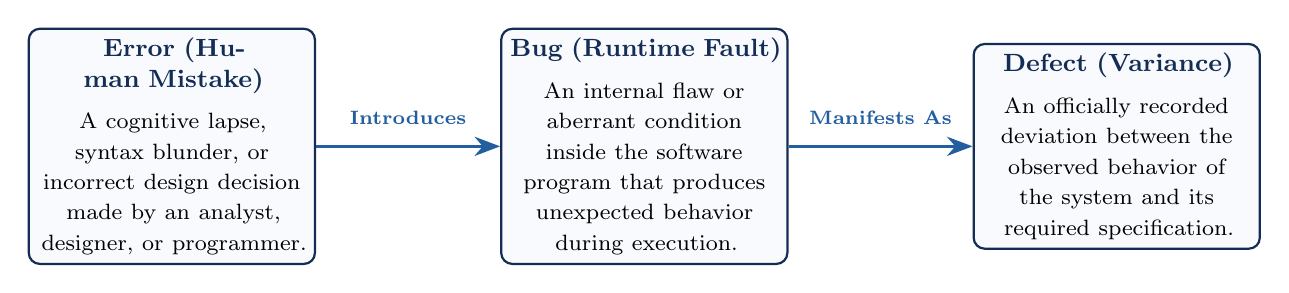
\begin{tikzpicture}[
    box/.style={rectangle, draw=primaryNavy, fill=lightBg, rounded corners=4pt, text width=3.4cm, minimum height=2.4cm, align=center, font=\small, thick},
    arrow/.style={-{Stealth[scale=1.1]}, very thick, color=secondaryBlue}
]
    \node[box] (error) at (1.8, 0) {\textbf{\color{primaryNavy}Error (Human Mistake)}\\\vspace{4pt}\footnotesize A cognitive lapse, syntax blunder, or incorrect design decision made by an analyst, designer, or programmer.};
    \node[box] (bug) at (7.8, 0) {\textbf{\color{primaryNavy}Bug (Runtime Fault)}\\\vspace{4pt}\footnotesize An internal flaw or aberrant condition inside the software program that produces unexpected behavior during execution.};
    \node[box] (defect) at (13.8, 0) {\textbf{\color{primaryNavy}Defect (Variance)}\\\vspace{4pt}\footnotesize An officially recorded deviation between the observed behavior of the system and its required specification.};

    \draw[arrow] (error.east) -- node[above=4pt, font=\scriptsize\bfseries, color=secondaryBlue] {Introduces} (bug.west);
    \draw[arrow] (bug.east) -- node[above=4pt, font=\scriptsize\bfseries, color=secondaryBlue] {Manifests As} (defect.west);
\end{tikzpicture}
\caption{The Defect Propagation Taxonomy: From Cognitive Error to Documented Defect.}
\label{fig:defect_taxonomy}
\end{figure}

\begin{conceptcard}{Formal Definitions in Quality Assurance}
\textbf{1. Error:} A human mistake or cognitive lapse made by a software developer, system analyst, or database architect. Examples include misinterpreting business logic, invoking an incorrect API signature, failing to account for null pointers, or introducing off-by-one boundary conditions in looping constructs.

\textbf{2. Bug:} An internal flaw, fault, or aberrant code state within an executable software artifact resulting directly from an underlying error. A bug represents the static physical existence of the error in compiled machine code or script text.

\textbf{3. Defect:} The formal variance or operational discrepancy identified when the actual runtime behavior of the software fails to match the expected outcome defined in the Software Requirement Specification (SRS). In professional workflows, defects are assigned unique tracking IDs, priority classifications, and lifecycle states within incident management databases.
\end{conceptcard}

\subsection{Strategic and Economic Importance of Quality Assurance}
The strategic importance of systematic testing is profoundly demonstrated by Barry Boehm's classical Software Defect Cost Incurrence Model. The cost required to remediate an error escalates exponentially as a project progresses through the lifecycle phases. An error caught during requirement analysis or architectural design carries a nominal remediation cost ($1\times$). That same error, if left undiscovered until unit testing, costs approximately $5\times$ to repair; during system testing, $10\times$; and if it escapes into operational production, the remediation cost escalates to between $30\times$ and $100\times$ due to data patching, hotfix engineering, emergency redeployment, regression auditing, customer compensation, and legal liabilities.

Beyond raw financial metrics, disciplined quality assurance underpins four institutional imperatives:
\begin{itemize}
    \item \textbf{Early Defect Isolation:} Preempting high-risk architectural failure modes before they become deeply intertwined with dependent codebases.
    \item \textbf{Customer Retention and Support Cost Containment:} Delivering predictable, defect-free experiences that prevent customer churn and reduce helpdesk ticket volumes.
    \item \textbf{Institutional Brand Protection:} Preventing high-profile public outages, data corruption scandals, and public relations crises that destroy enterprise value.
    \item \textbf{Regulatory Compliance and Attack Surface Hardening:} Guaranteeing conformity with international digital standards (e.g., ISO/IEC 25010) and closing attack vectors before adversaries exploit them.
\end{itemize}

\subsection{Comprehensive System Testing Taxonomy}
Quality assurance encompasses a multi-tiered hierarchy of testing modalities, each calibrated to evaluate distinct architectural layers and quality attributes:

\begin{table}[htbp]
\centering
\small
\renewcommand{\arraystretch}{1.25}
\begin{tabularx}{\textwidth}{L{2.5cm} L{3.2cm} Y L{3.2cm}}
\toprule
\rowcolor{tableHeader}
\textbf{Testing Modality} & \textbf{Primary Scope} & \textbf{Architectural Objective} & \textbf{Target Environment} \\
\midrule
\textbf{Unit Testing} & Individual subroutines, methods, classes & Verify internal algorithmic accuracy, conditional branches, and arithmetic operations in complete isolation. & Local Developer Workstation / Isolated CI Runner \\
\textbf{Integration Testing} & Inter-module boundaries, API contracts & Expose interface mismatches, type marshaling errors, communication protocol failures, and shared-state bugs. & Dedicated CI Pipeline / Shared Integration Server \\
\textbf{System Testing} & Fully assembled application stack & Validate end-to-end business workflows, persistence pipelines, and total system behavior against the SRS. & Production Mirror / Pre-Release Staging Sandbox \\
\textbf{Acceptance Testing} & End-to-end operational use cases & Obtain formal sign-off from business stakeholders; encompasses Alpha (developer-supervised) and Beta (field user) trials. & Controlled Client Environment / Production Sandbox \\
\textbf{Regression Testing} & Complete or risk-weighted test suites & Ensure that recent bug fixes, code refactoring, or dependency updates have not degraded preexisting functionality. & Automated Continuous Integration (CI) Fleet \\
\textbf{Performance Testing} & Hardware resources, network, DB throughput & Quantify response latency, concurrency thresholds, and degradation limits under Load, Stress, and Soak testing. & Isolated High-Capacity Performance Lab \\
\textbf{Security Testing} & Authentication, cryptographic boundaries & Detect vulnerabilities, access control bypasses, SQL injection, cross-site scripting (XSS), and zero-day exposure. & Isolated Security Penetration Testing Sandbox \\
\bottomrule
\end{tabularx}
\caption{Comprehensive Software Testing Taxonomy Across the Engineering Lifecycle.}
\label{tab:testing_taxonomy}
\end{table}

\subsection{Standardized Test Plan Artifact Architecture}
A Test Plan is an indispensable formal artifact that establishes execution discipline, traceability, and institutional accountability. Without a standardized template, testing devolves into ad-hoc experimentation that lacks repeatability. A rigorous test plan structure contains metadata, case identifiers, a parameter grid, execution scripts, and recorded observations:

\begin{figure}[htbp]
\centering
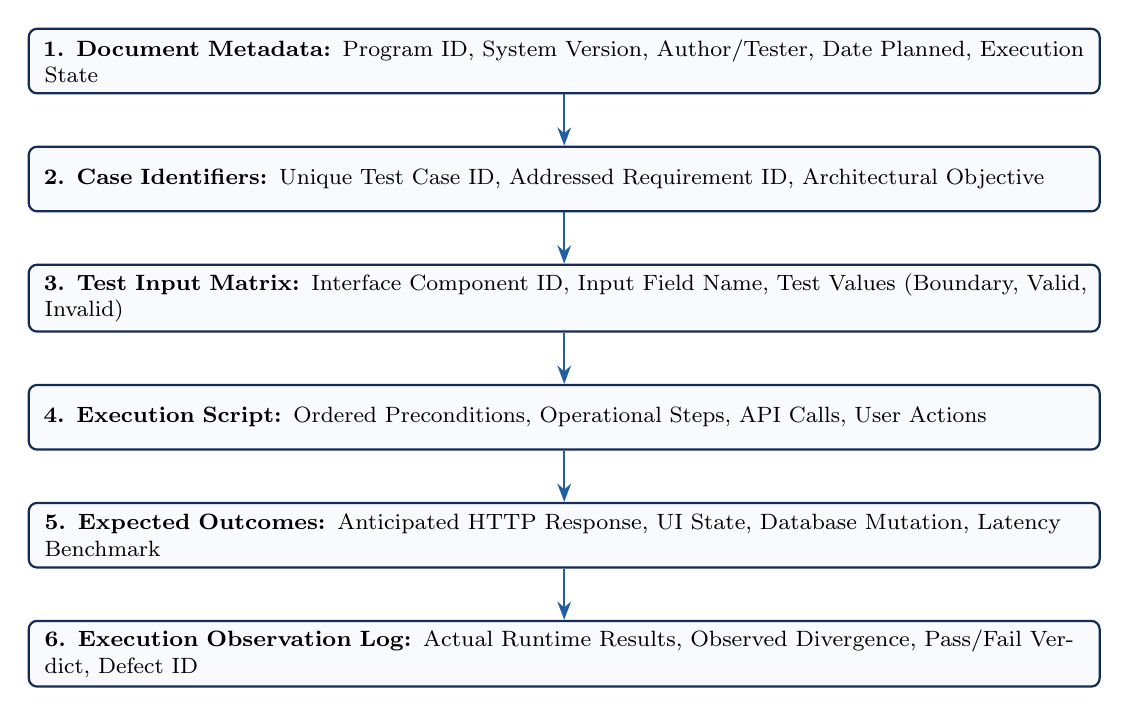
\begin{tikzpicture}[
    node distance=0.65cm,
    block/.style={rectangle, draw=primaryNavy, fill=lightBg, rounded corners=3pt, minimum width=13.6cm, text width=13.2cm, minimum height=0.82cm, align=left, font=\footnotesize, thick},
    arrow/.style={-{Stealth[scale=1.0]}, thick, color=secondaryBlue}
]
    \node[block] (meta) {\textbf{1. Document Metadata:} Program ID, System Version, Author/Tester, Date Planned, Execution State};
    \node[block, below=of meta] (ident) {\textbf{2. Case Identifiers:} Unique Test Case ID, Addressed Requirement ID, Architectural Objective};
    \node[block, below=of ident] (matrix) {\textbf{3. Test Input Matrix:} Interface Component ID, Input Field Name, Test Values (Boundary, Valid, Invalid)};
    \node[block, below=of matrix] (script) {\textbf{4. Execution Script:} Ordered Preconditions, Operational Steps, API Calls, User Actions};
    \node[block, below=of script] (expect) {\textbf{5. Expected Outcomes:} Anticipated HTTP Response, UI State, Database Mutation, Latency Benchmark};
    \node[block, below=of expect] (actual) {\textbf{6. Execution Observation Log:} Actual Runtime Results, Observed Divergence, Pass/Fail Verdict, Defect ID};

    \draw[arrow] (meta) -- (ident);
    \draw[arrow] (ident) -- (matrix);
    \draw[arrow] (matrix) -- (script);
    \draw[arrow] (script) -- (expect);
    \draw[arrow] (expect) -- (actual);
\end{tikzpicture}
\caption{Hierarchical Architecture of a Standardized Enterprise Test Plan Document.}
\label{fig:test_plan_architecture}
\end{figure}

To illustrate the concrete application of this artifact, Table~\ref{tab:test_plan_specimen} provides a complete, production-grade specimen for verifying user authentication and credential security.

\begin{table}[htbp]
\centering
\footnotesize
\renewcommand{\arraystretch}{1.2}
\begin{tabularx}{\textwidth}{|L{3.1cm}|L{2.9cm}|L{4.3cm}|Y|}
\hline
\rowcolor{tableHeader}
\multicolumn{4}{|c|}{\textbf{\normalsize FORMAL SOFTWARE TEST PLAN EXECUTION SHEET}} \\
\hline
\textbf{Program / Module ID:} & AUTH-MOD-042 & \textbf{Date Designed:} & 2026-10-25 \\
\textbf{Software Version:} & v2.4.0-RC1 & \textbf{Date Conducted:} & 2026-10-25 \\
\textbf{Tester Name:} & SQA Lead Engineer & \textbf{Overall Verdict:} & PASSED (Conditional) \\
\hline
\textbf{Test Case ID:} & TC-AUTH-008 & \textbf{Requirement Addressed:} & SRS-SEC-014 (MFA Enforcement) \\
\hline
\textbf{Test Objective:} & \multicolumn{3}{>{\raggedright\arraybackslash}p{\dimexpr\textwidth-3.1cm-4\tabcolsep-3\arrayrulewidth\relax}|}{Verify that accounts with Multi-Factor Authentication (MFA) enabled reject valid primary credentials when provided with an invalid or expired Time-Based One-Time Password (TOTP) token.} \\
\hline
\rowcolor{lightBg}
\multicolumn{4}{|c|}{\textbf{Test Input Matrix and Parameter Grid}} \\
\hline
\textbf{Target Interface ID} & \textbf{Data Field Name} & \textbf{Test Value Entered} & \textbf{Input Classification} \\
\hline
UI-LOGIN-FLD-01 & \texttt{user\_identity} & \texttt{anika.amzad@}\allowbreak\texttt{kyau.edu.bd} & Valid Production Email \\
UI-LOGIN-FLD-02 & \texttt{user\_password} & \texttt{Str0ngP@ss}\allowbreak\texttt{w0rd!2026} & Valid Cryptographic Hash \\
UI-LOGIN-FLD-03 & \texttt{mfa\_totp\_code} & \texttt{000000} (Deliberate invalid) & Invalid / Spoofed Token \\
UI-LOGIN-FLD-03 & \texttt{mfa\_totp\_code} & \texttt{849201} (Expired 90s prior) & Expired Token \\
\hline
\rowcolor{lightBg}
\multicolumn{4}{|c|}{\textbf{Execution Script, Expected Outcomes, and Observed Deviations}} \\
\hline
\multicolumn{4}{|>{\raggedright\arraybackslash}p{\dimexpr\textwidth-2\tabcolsep-2\arrayrulewidth\relax}|}{\textbf{Step-by-Step Execution Script:} \newline
1. Navigate to endpoint \texttt{/auth/login} using HTTPS. \newline
2. Inject valid credentials into fields \texttt{user\_identity} and \texttt{user\_password}; submit form. \newline
3. Confirm system transitions state to \texttt{CHALLENGE\_MFA} and displays modal dialog. \newline
4. Inject \texttt{000000} into the token field and press \texttt{Verify}. \newline
5. Observe HTTP response status code, JSON error payload, and front-end alert rendering.} \\
\hline
\textbf{Expected Results:} & \multicolumn{3}{>{\raggedright\arraybackslash}p{\dimexpr\textwidth-3.1cm-4\tabcolsep-3\arrayrulewidth\relax}|}{System must return HTTP 401 Unauthorized, payload \texttt{\{"error":} \texttt{"INVALID\_}\allowbreak\texttt{MFA\_TOKEN"\}}, increment failed attempt counter by 1, and prompt user with ``Invalid security token.''} \\
\hline
\textbf{Observed Results:} & \multicolumn{3}{>{\raggedright\arraybackslash}p{\dimexpr\textwidth-3.1cm-4\tabcolsep-3\arrayrulewidth\relax}|}{HTTP 401 returned. Token rejected. Counter incremented accurately. No session cookie emitted. Observed behavior matches SRS-SEC-014 completely.} \\
\hline
\end{tabularx}
\caption{Production-Grade Standardized Test Plan Artifact Specimen.}
\label{tab:test_plan_specimen}
\end{table}

\subsection{Systemic Operational Challenges in Testing}
Software testing is rarely constrained by tooling alone; rather, it is shaped by five systemic operational friction points:
\begin{enumerate}
    \item \textbf{System Complexity and Non-Deterministic Interdependencies:} Modern applications consist of microservices, asynchronous message queues, distributed databases, and third-party APIs. When an error manifests, isolating the root cause from a web of cascading timeouts and retries is difficult.
    \item \textbf{Severe Resource and Schedule Compression:} Testing cycles are routinely compressed at the end of release schedules. When upstream coding slips, QA teams face severe time pressure, often leading to curtailed regression testing.
    \item \textbf{Requirement Volatility:} In agile environments, stakeholder requirements frequently shift during mid-sprint cycles. Rapid requirement churn invalidates previously written test automation suites, creating substantial test-maintenance debt.
    \item \textbf{Toolchain Fragmentation and Framework Selection Dilemmas:} The test automation ecosystem is fragmented into commercial tools, open-source frameworks, and custom internal libraries. Choosing the wrong automation framework leads to brittle scripts that break on minor DOM alterations.
    \item \textbf{Cross-Functional Communication Breakdowns:} Organizational silos between development, QA, and business stakeholders lead to adversarial interactions, where defects are disputed rather than collaboratively remediated.
\end{enumerate}

% =========================================================================
% SECTION 3: INTEGRATION TESTING METHODOLOGIES & ARCHITECTURAL APPROACHES
% =========================================================================
\section[Integration Testing Methodologies]{Integration Testing Methodologies and Architectural Approaches}
\label{sec:integration_testing}

\subsection{Architectural Concept and Engineering Rationale}
Integration testing is the disciplined verification of the interactions, data exchanges, and interface contracts among integrated software components. While unit testing proves that a mathematical function calculates accurately in an isolated runtime harness, integration testing proves whether that function can serialize its result into JSON, transmit it across an RPC socket, authenticate through a gateway, and commit state to a remote database transaction.

The engineering rationale for integration testing stems from interface fragility. Subsystems may function correctly in isolation yet fail catastrophically when coupled. Common points of failure include:
\begin{itemize}
    \item \textbf{Data Format and Type Mismatches:} An upstream service transmitting dates in Unix epoch timestamps while the downstream consumer expects ISO-8601 string formatting.
    \item \textbf{Protocol and Schema Drift:} Silent API drift where an unannounced optional field becomes mandatory, causing deserialization crashes.
    \item \textbf{Concurrency and Race Conditions:} Asynchronous operations where a database record is queried by Service~B before Service~A's asynchronous write completes.
    \item \textbf{Resource Contention:} Multiple worker threads deadlocking on shared socket pools or database connection limits.
\end{itemize}

\subsection{Concrete Real-World Domain Examples}
To ground these concepts in enterprise realities, consider two representative system workflows:

\textbf{1. The E-Commerce Checkout Pipeline:} In an enterprise digital storefront, the checkout transaction spans four independent services: the \textit{User Authentication Service}, the \textit{Product Inventory Catalog}, the \textit{Shopping Cart State Manager}, and the external \textit{Payment Gateway Processor}. During integration testing, the quality assurance framework must verify that:
\begin{itemize}
    \item When a customer authorizes a \$150 purchase, the Payment Gateway generates an authorization token that is verified by the Order Service.
    \item The Inventory Service places a reservation lock on the specific stock-keeping unit (SKU), preventing double-allocation race conditions from concurrent buyers.
    \item If the external payment provider encounters a gateway timeout, the transaction rolls back across all services, ensuring the shopping cart remains populated and the stock reservation is released.
\end{itemize}

\textbf{2. Core Banking Fund Transfer:} In financial transaction processing, a single inter-account transfer demands atomic coordination across the \textit{Customer Ledger Service}, the \textit{Fraud Detection Engine}, the \textit{Notification Gateway}, and the central \textit{Core Accounting Database}. Integration testing validates that:
\begin{itemize}
    \item The debit from Account~A and the credit to Account~B execute within a single distributed two-phase commit (2PC) or SAGA transaction.
    \item A transient failure in the Notification Gateway (SMS/Email) does not trigger an erroneous rollback of the financial transfer.
    \item High transaction concurrency does not produce balance inconsistencies or negative ledger balances under network latency.
\end{itemize}

\subsection{Comparative Analysis of Architectural Integration Strategies}
Organizations typically employ one of four primary architectural strategies to assemble and test multi-module systems:

\begin{figure}[htbp]
\centering
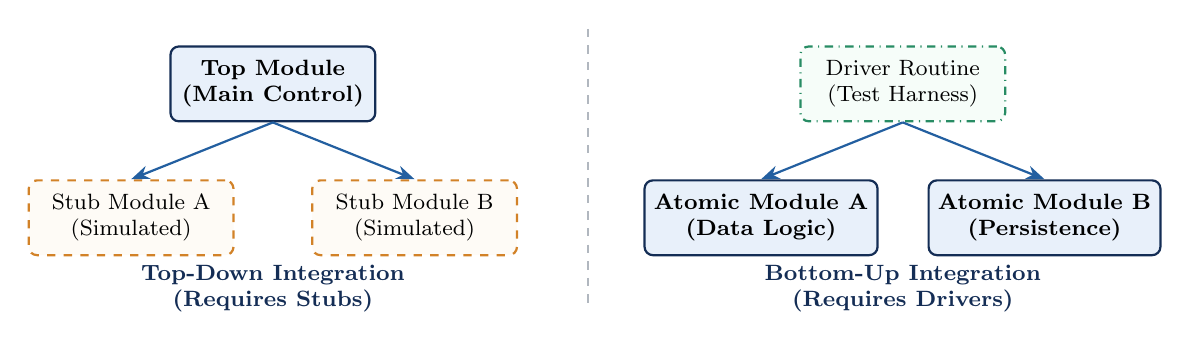
\begin{tikzpicture}[
    module/.style={rectangle, draw=primaryNavy, fill=tableHeader, rounded corners=3pt, minimum width=2.6cm, minimum height=0.95cm, align=center, font=\footnotesize\bfseries, thick},
    stub/.style={rectangle, draw=caseBorder, fill=caseBg, dashed, rounded corners=3pt, minimum width=2.6cm, minimum height=0.95cm, align=center, font=\footnotesize, thick},
    driver/.style={rectangle, draw=auditBorder, fill=auditBg, dashdotted, rounded corners=3pt, minimum width=2.6cm, minimum height=0.95cm, align=center, font=\footnotesize, thick},
    arrow/.style={-{Stealth[scale=1.0]}, thick, color=secondaryBlue}
]
    % Panel Left: Top-Down
    \node[module] (topM1) at (0, 2.4) {Top Module\\(Main Control)};
    \node[stub] (stubM2) at (-1.8, 0.7) {Stub Module A\\(Simulated)};
    \node[stub] (stubM3) at (1.8, 0.7) {Stub Module B\\(Simulated)};
    \draw[arrow] (topM1.south) -- (stubM2.north);
    \draw[arrow] (topM1.south) -- (stubM3.north);
    \node[font=\footnotesize\bfseries\color{primaryNavy}, align=center] at (0, -0.2) {Top-Down Integration\\(Requires Stubs)};

    % Separator Line
    \draw[dashed, color=slateGray!40, thick] (4.0, 3.1) -- (4.0, -0.4);

    % Panel Right: Bottom-Up
    \node[driver] (drvM1) at (8.0, 2.4) {Driver Routine\\(Test Harness)};
    \node[module] (botM2) at (6.2, 0.7) {Atomic Module A\\(Data Logic)};
    \node[module] (botM3) at (9.8, 0.7) {Atomic Module B\\(Persistence)};
    \draw[arrow] (drvM1.south) -- (botM2.north);
    \draw[arrow] (drvM1.south) -- (botM3.north);
    \node[font=\footnotesize\bfseries\color{primaryNavy}, align=center] at (8.0, -0.2) {Bottom-Up Integration\\(Requires Drivers)};
\end{tikzpicture}
\caption{Architectural Harness Requirements: Stubs in Top-Down versus Drivers in Bottom-Up Integration.}
\label{fig:stubs_and_drivers}
\end{figure}

\begin{enumerate}
    \item \textbf{Big Bang Integration:} In this uncoordinated approach, all developing software modules are compiled independently and then coupled simultaneously into a single monolithic whole for execution.
    \begin{itemize}
        \item \textit{Operational Assessment:} Extreme risk. When fatal runtime faults or memory corruptions occur, pinpointing the culprit module is difficult because faults cascade across untested boundaries. It is suitable only for tiny, trivial applications.
    \end{itemize}
    \item \textbf{Top-Down Integration:} Testing begins at the highest architectural level (e.g., the primary user interface or controller router) and progresses downward through the module call hierarchy.
    \begin{itemize}
        \item \textit{Harness Dependency:} Lower-level modules that have not yet been coded or integrated must be substituted with \textbf{Stubs}---dummy subroutines that mimic lower-level functionality by returning fixed, hardcoded responses.
        \item \textit{Strategic Trade-off:} Validates core business flows and executive logic early; however, low-level data access and complex utility bugs remain unverified until the end of the project.
    \end{itemize}
    \item \textbf{Bottom-Up Integration:} Testing commences at the foundation of the architecture (e.g., database abstraction layers, mathematical libraries, file utilities) and ascends upward.
    \begin{itemize}
        \item \textit{Harness Dependency:} Higher-level controlling modules that are not yet integrated are substituted with \textbf{Drivers}---specialized test scripts and calling harnesses that invoke lower-level routines with test inputs.
        \item \textit{Strategic Trade-off:} Thoroughly verifies critical data algorithms, file handling, and database transactions early; however, high-level structural design flaws and workflow breakdowns are discovered late.
    \end{itemize}
    \item \textbf{Incremental / Sandwich Integration:} A hybrid engineering paradigm where the system is partitioned into a central functional core. Bottom-up integration is applied to foundational utility layers, while top-down integration is applied to user-facing orchestration layers, converging on the middle layer.
\end{enumerate}

\begin{table}[htbp]
\centering
\small
\renewcommand{\arraystretch}{1.25}
\begin{tabularx}{\textwidth}{L{2.5cm} L{3.2cm} Y L{3.2cm}}
\toprule
\rowcolor{tableHeader}
\textbf{Integration Strategy} & \textbf{Test Harness Needs} & \textbf{Primary Advantages} & \textbf{Key Disadvantages} \\
\midrule
\textbf{Big Bang} & Minimal / None & No overhead developing stubs or drivers; straightforward for trivial programs. & Catastrophic defect localization; debugging is slow and high-risk. \\
\textbf{Top-Down} & Requires extensive \textbf{Stubs} & Major architectural flaws caught early; demonstrates system feasibility to clients. & Low-level data utility bugs discovered late; building stubs requires substantial effort. \\
\textbf{Bottom-Up} & Requires extensive \textbf{Drivers} & Core mathematical, data, and persistence layers thoroughly hardened early. & Architectural logic and user interface validated late; driver development adds overhead. \\
\textbf{Incremental (Sandwich)} & Balanced mix of Stubs and Drivers & Parallel testing across teams; combines top-level validation with bottom-tier rigor. & Higher architectural coordination required; complex configuration management. \\
\bottomrule
\end{tabularx}
\caption{Comparative Architectural Matrix of Integration Testing Strategies.}
\label{tab:integration_matrix}
\end{table}

\subsection{Error Discovery Rate Dynamics Across the SDLC}
Empirical software metrics indicate that the frequency of defect discovery does not remain constant throughout the software development lifecycle. Instead, it follows a distinct curve characterized by a moderate starting rate during Unit Testing, a sharp zenith during Integration Testing, and a gradual decay through subsequent validation stages.

\begin{figure}[htbp]
\centering
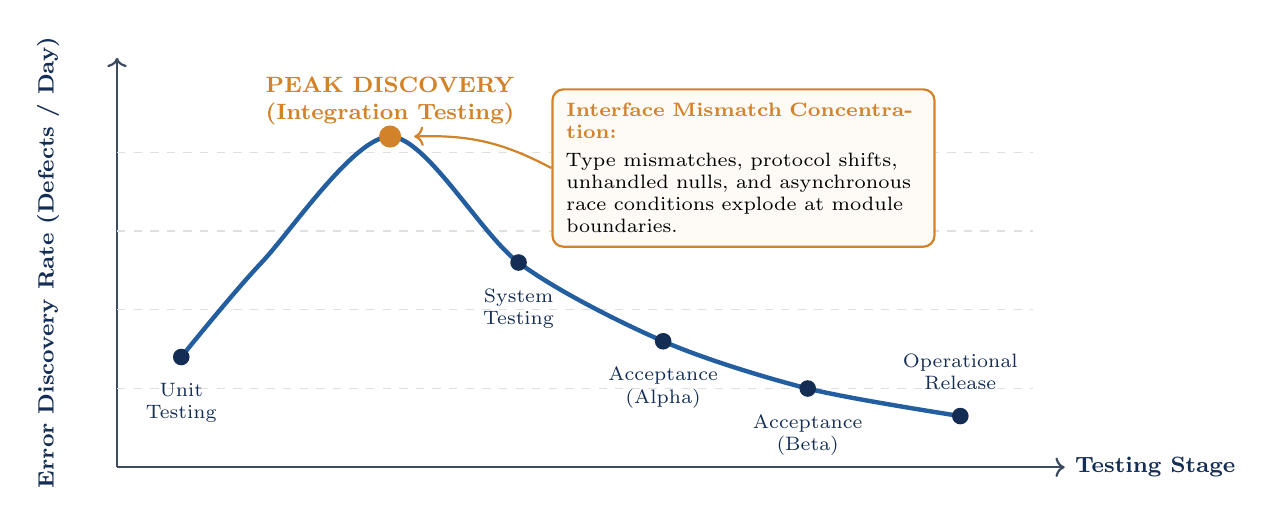
\begin{tikzpicture}[x=1.02cm, y=1.0cm]
    % Axes
    \draw[->, thick, color=slateGray] (0,0) -- (11.8,0) node[right, font=\footnotesize\bfseries, color=primaryNavy] {Testing Stage};
    \draw[->, thick, color=slateGray] (0,0) -- (0,5.2);
    \node[rotate=90, font=\footnotesize\bfseries, color=primaryNavy, anchor=south] at (-0.6, 2.6) {Error Discovery Rate (Defects / Day)};

    % Horizontal grid lines
    \draw[dashed, color=gray!25] (0,1) -- (11.4,1);
    \draw[dashed, color=gray!25] (0,2) -- (11.4,2);
    \draw[dashed, color=gray!25] (0,3) -- (11.4,3);
    \draw[dashed, color=gray!25] (0,4) -- (11.4,4);

    % Bell Curve Path
    \draw[ultra thick, color=secondaryBlue, smooth] 
        plot coordinates {(0.8, 1.4) (1.8, 2.6) (3.4, 4.2) (5.0, 2.6) (6.8, 1.6) (8.6, 1.0) (10.5, 0.65)};

    % Key Stage Points
    \fill[color=primaryNavy] (0.8, 1.4) circle (3pt) node[below=6pt, font=\scriptsize, align=center] {Unit\\Testing};
    \fill[color=caseBorder] (3.4, 4.2) circle (4pt);
    \node[font=\footnotesize\bfseries, color=caseBorder, align=center] at (3.4, 4.65) {PEAK DISCOVERY\\(Integration Testing)};
    \fill[color=primaryNavy] (5.0, 2.6) circle (3pt) node[below=6pt, font=\scriptsize, align=center] {System\\Testing};
    \fill[color=primaryNavy] (6.8, 1.6) circle (3pt) node[below=6pt, font=\scriptsize, align=center] {Acceptance\\(Alpha)};
    \fill[color=primaryNavy] (8.6, 1.0) circle (3pt) node[below=6pt, font=\scriptsize, align=center] {Acceptance\\(Beta)};
    \fill[color=primaryNavy] (10.5, 0.65) circle (3pt) node[above=6pt, font=\scriptsize, align=center] {Operational\\Release};

    % Callout Box positioned clearly in upper right quadrant
    \node[draw=caseBorder, fill=caseBg, rounded corners=4pt, text width=4.5cm, font=\scriptsize, inner sep=5pt, thick] (callout) at (7.8, 3.8) {
        \textbf{\color{caseBorder}Interface Mismatch Concentration:}\vspace{2pt}\\
        Type mismatches, protocol shifts, unhandled nulls, and asynchronous race conditions explode at module boundaries.
    };
    \draw[->, thick, color=caseBorder] (callout.west) to[bend right=15] (3.7, 4.2);
\end{tikzpicture}
\caption{Mathematical Profile of Error Discovery Rates Across Sequential Testing Phases.}
\label{fig:error_discovery_curve}
\end{figure}

The engineering rationale for this distribution is clear:
\begin{itemize}
    \item \textbf{Unit Testing Phase:} Unit testing exhibits a moderate defect rate because it isolates local syntax errors, boundary violations, and localized branching flaws within single classes. The scope is bounded, and external interactions are mocked out.
    \item \textbf{Integration Testing Peak:} When disparate modules are coupled, the system experiences an explosion of variable states. Mismatched database assumptions, uncoordinated null handling, thread concurrency contention, and protocol drifts concentrate heavily at component boundaries. Consequently, this stage yields the \textit{absolute peak} in discovered defects.
    \item \textbf{Decay Across System and Acceptance Testing:} By the time the software advances to system-level and user acceptance suites, structural boundary defects have largely been remediated. The defect discovery curve decays into a long tail, uncovering rare race conditions, edge-case usability flaws, and unexpected infrastructure friction points.
\end{itemize}

% =========================================================================
% SECTION 4: SDLC EXECUTION & OPERATIONAL CHALLENGES
% =========================================================================
\section[SDLC Execution and Challenges]{Software Development Life Cycle Execution and Operational Challenges}
\label{sec:sdlc_execution}

\subsection{Foundational SDLC Phases}
The Software Development Life Cycle (SDLC) is the institutional framework that structures the engineering of software systems from inception to retirement:
\begin{enumerate}
    \item \textbf{Requirements Analysis and Specification:} Gathering stakeholder needs, documenting use cases, and creating the Software Requirements Specification (SRS) artifact.
    \item \textbf{Architectural and System Design:} Formulating high-level system topology (microservices, monoliths), database schemas (ER diagrams), API contracts, and security boundaries.
    \item \textbf{Implementation (Coding):} Translating design specifications into executable source code adhering to established styling and modularization principles.
    \item \textbf{Verification and Testing:} Executing unit, integration, system, and regression test suites to validate functional correctness and isolate defects.
    \item \textbf{Deployment and Staging:} Packaging compiled code, provisioning target infrastructure, executing schema migrations, and promoting code to production.
    \item \textbf{Maintenance and Evolution:} Ongoing monitoring, patching, performance tuning, and accommodating shifting business requirements throughout operational life.
\end{enumerate}

\subsection{Systemic Development and Deployment Friction Points}
Transitioning code from development workstations into operational production introduces significant technical and organizational friction:
\begin{itemize}
    \item \textbf{The Environmental Drift Dilemma (``Works on My Machine''):} Discrepancies between local developer laptops, staging sandboxes, and production servers (differing OS kernels, patch levels, or unannounced dependency updates) cause unpredictable runtime faults.
    \item \textbf{Persistent Data Schema Synchronization:} Deploying code modifications that require non-backward-compatible database mutations without locking production tables or causing downtime.
    \item \textbf{Distributed Secret Management:} Safely injecting production credentials, API access keys, and TLS certificates without committing secrets to version control repositories.
    \item \textbf{External and Regulatory Volatility:} Rapid shifts in data privacy legislation (e.g., GDPR, CCPA), evolving industry security mandates, and breaking changes in underlying third-party cloud SDKs and hardware architectures.
\end{itemize}

\subsection{The Staging and SDLC Execution Pipeline}
To move software reliably from local developer environments to operational production, organizations rely on a multi-stage execution pipeline:

\begin{figure}[htbp]
\centering
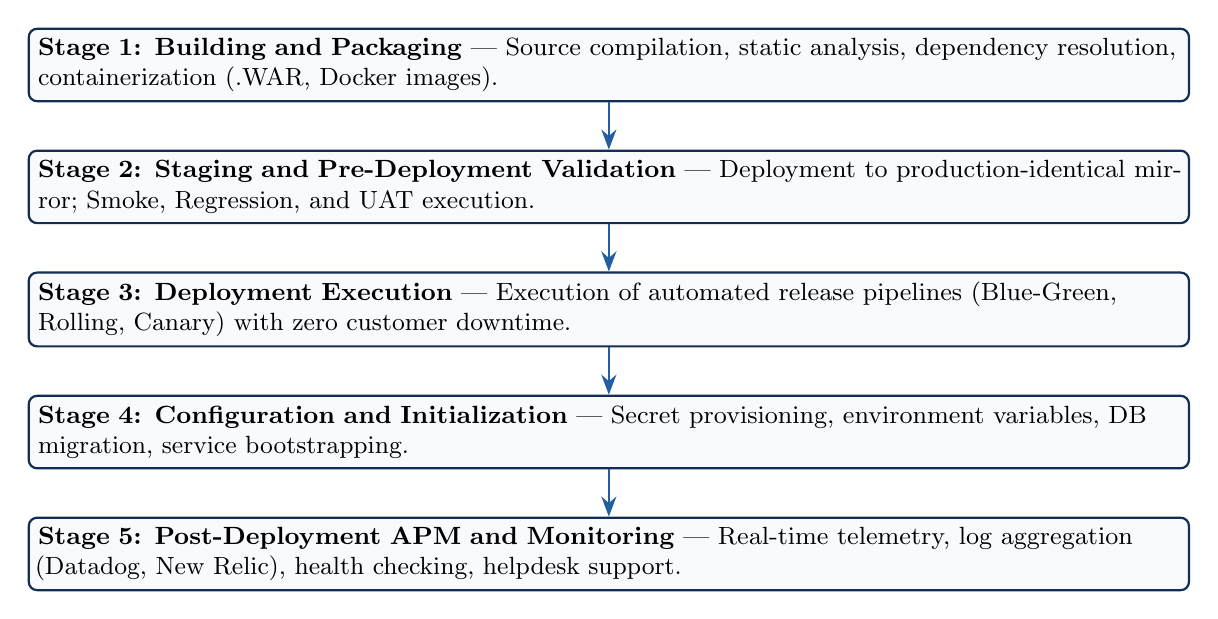
\begin{tikzpicture}[
    node distance=0.6cm,
    stage/.style={rectangle, draw=primaryNavy, fill=lightBg, rounded corners=3pt, text width=14.5cm, minimum height=0.92cm, font=\small, thick, align=left},
    arrow/.style={-{Stealth[scale=1.1]}, thick, color=secondaryBlue}
]
    \node[stage] (s1) {\textbf{Stage 1: Building and Packaging} --- Source compilation, static analysis, dependency resolution, containerization (.WAR, Docker images).};
    \node[stage, below=of s1] (s2) {\textbf{Stage 2: Staging and Pre-Deployment Validation} --- Deployment to production-identical mirror; Smoke, Regression, and UAT execution.};
    \node[stage, below=of s2] (s3) {\textbf{Stage 3: Deployment Execution} --- Execution of automated release pipelines (Blue-Green, Rolling, Canary) with zero customer downtime.};
    \node[stage, below=of s3] (s4) {\textbf{Stage 4: Configuration and Initialization} --- Secret provisioning, environment variables, DB migration, service bootstrapping.};
    \node[stage, below=of s4] (s5) {\textbf{Stage 5: Post-Deployment APM and Monitoring} --- Real-time telemetry, log aggregation (Datadog, New Relic), health checking, helpdesk support.};

    \draw[arrow] (s1) -- (s2);
    \draw[arrow] (s2) -- (s3);
    \draw[arrow] (s3) -- (s4);
    \draw[arrow] (s4) -- (s5);
\end{tikzpicture}
\caption{The Five-Stage Staging and SDLC Release Pipeline.}
\label{fig:sdlc_pipeline}
\end{figure}

\begin{conceptcard}{Detailed Breakdown of Pipeline Stages}
\textbf{1. Building and Packaging:} Source code is compiled, linked, and bundled alongside necessary configuration files, runtime environments, and schema migration scripts. In Java enterprise environments, this yields an immutable Web Application Archive (\texttt{.WAR}) or an Enterprise Archive (\texttt{.EAR}); in cloud-native paradigms, this yields an encrypted Open Container Initiative (OCI) Docker container image with cryptographic checksums.

\textbf{2. Staging and Pre-Deployment Testing:} The packaged artifact is deployed into a dedicated Staging Environment that mirrors the exact hardware topologies, database sizes, operating systems, and network configurations of production. Here, three testing suites execute:
\begin{itemize}
    \item \textit{Smoke Testing (Sanity Check):} A brief suite verifying that the application launches, binds to network ports, connects to database instances, and renders core home interfaces.
    \item \textit{Staging Regression Testing:} Broad automated suites verifying end-to-end integration across all dependent modules.
    \item \textit{User Acceptance Testing (UAT):} Business analysts and end-users validate actual operational workflows for formal release sign-off.
\end{itemize}

\textbf{3. Deployment Execution:} Automated orchestration engines (e.g., Kubernetes, Terraform, Ansible) execute the selected release pattern to deploy the tested build into the live cluster.

\textbf{4. Configuration and Initialization:} The runtime environment is populated with target environment variables, secrets (API tokens, database credentials fetched from HashiCorp Vault), schema migrations are committed against the persistence tier, and application worker pools are initialized.

\textbf{5. Post-Deployment Monitoring and Support:} Live traffic is monitored using Application Performance Monitoring (APM) platforms to track response latencies, error frequencies, and server resource utilization, backed by customer support channels for rapid escalation.
\end{conceptcard}

% =========================================================================
% SECTION 5: DEPLOYMENT STRATEGIES & OPERATIONAL PATTERNS
% =========================================================================
\section[Deployment Strategies]{Deployment Strategies, Patterns, and Initialization Protocols}
\label{sec:deployment_strategies}

\subsection{Architectural Trade-Off Analysis}
In modern system administration, the method used to deploy software into production fundamentally determines service availability, operational risk, and infrastructure costs. Deploying is no longer an all-or-nothing proposition where engineers accept scheduled multi-hour outages. Instead, software engineers select from seven distinct deployment patterns, each tailored to specific risk tolerances, budgets, and architectural constraints:

\begin{table}[htbp]
\centering
\footnotesize
\renewcommand{\arraystretch}{1.25}
\begin{tabularx}{\textwidth}{L{2.0cm} Y L{1.8cm} L{1.6cm} L{3.0cm}}
\toprule
\rowcolor{tableHeader}
\textbf{Pattern Name} & \textbf{Operational Mechanism} & \textbf{Downtime} & \textbf{Risk Level} & \textbf{Typical Domain Fit} \\
\midrule
\textbf{Recreate} & Terminate all Version~1 instances completely; provision and launch Version~2 fleet. & Significant & High & Non-critical internal tools, batch processors, dev sandboxes. \\
\textbf{Rolling} & Incrementally replace subsets (e.g., 20\%) of Version~1 nodes with Version~2 behind a load balancer. & Zero to Minimal & Moderate & Stateless web services, horizontally scaled microservice clusters. \\
\textbf{Blue-Green} & Run two identical production clusters; switch active router/DNS traffic from Blue to Green. & Zero & Low & Mission-critical banking, core healthcare systems, ERP suites. \\
\textbf{Canary} & Route a tiny traffic fraction (e.g., 5\%) to Version~2; expand to 100\% only after telemetry verification. & Zero & Very Low & Global consumer platforms, SaaS products, social media networks. \\
\textbf{A/B Testing} & Route distinct user demographics to Variant~A or Variant~B to measure behavioral/conversion metrics. & Zero & Low & E-commerce checkout funnels, marketing optimizations, UI redesigns. \\
\textbf{Shadow} & Duplicate incoming live production traffic asynchronously to Version~2; discard responses. & Zero & Minimal & High-frequency algorithmic trading, ML models, core database engines. \\
\textbf{Feature Toggles} & Deploy dormant code behind conditional feature flags; enable dynamically at runtime. & Zero & Minimal & Continuous integration, Trunk-Based Development, targeted rollouts. \\
\bottomrule
\end{tabularx}
\caption{Comprehensive Architectural Trade-off Matrix of Enterprise Deployment Strategies.}
\label{tab:deployment_matrix}
\end{table}

\subsection{Exposition of Deployment Patterns}
\textbf{1. Recreate Deployment:} The simplest and most primitive strategy. The operational infrastructure hosting Version~1 is shut down simultaneously, dropping all active connections. Version~2 is subsequently deployed, initialized, and started.
\begin{itemize}
    \item \textit{Evaluation:} While it avoids the challenge of running two different versions concurrently against a shared database, it forces guaranteed service downtime and carries a high risk of extended outages if Version~2 fails during startup.
\end{itemize}

\textbf{2. Rolling Deployment:} An incremental deployment mechanism where worker nodes across a cluster are updated in rolling batches (e.g., 25\% at a time). As each batch successfully passes health-check probes, the load balancer routes traffic to it while terminating nodes running the legacy version.
\begin{itemize}
    \item \textit{Evaluation:} Enables zero downtime without requiring a complete doubling of underlying hardware capacity. However, it requires that the database schema remain backward-compatible, as Version~1 and Version~2 execute concurrently during the rollout window.
\end{itemize}

\textbf{3. Blue-Green Deployment:} A zero-downtime release paradigm that provisions two identical, independent physical or virtual production environments: the currently live environment (Blue) and the idle, pre-production environment (Green). Version~2 is deployed and tested on Green without impacting live users. Once certified, the network load balancer or ingress router switches traffic to Green.
\begin{itemize}
    \item \textit{Evaluation:} Provides instantaneous switchover and near-instantaneous rollback: if an anomaly occurs on Green, the router simply reverts traffic to Blue. Its primary drawback is cost, as it requires doubling infrastructure capacity during the deployment window.
\end{itemize}

\begin{figure}[htbp]
\centering
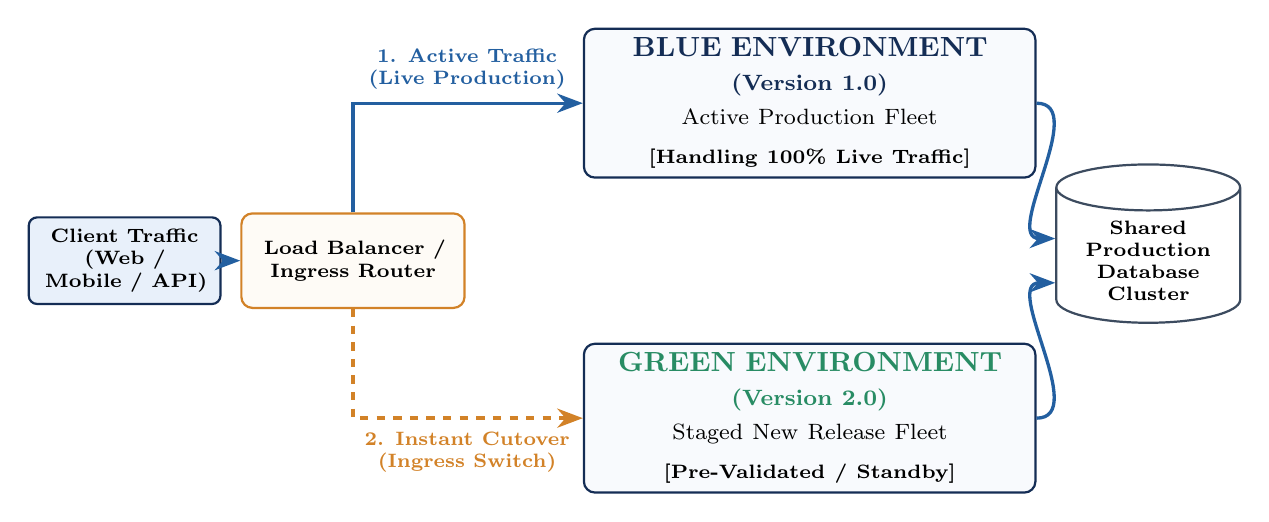
\begin{tikzpicture}[
    client/.style={rectangle, draw=primaryNavy, fill=tableHeader, rounded corners=3pt, text width=2.2cm, minimum height=1.1cm, align=center, font=\scriptsize\bfseries, thick},
    lb/.style={rectangle, draw=caseBorder, fill=caseBg, rounded corners=4pt, text width=2.6cm, minimum height=1.2cm, align=center, font=\scriptsize\bfseries, thick},
    envBox/.style={rectangle, draw=primaryNavy, fill=lightBg, rounded corners=4pt, text width=5.5cm, minimum height=1.8cm, align=center, thick},
    db/.style={cylinder, shape border rotate=90, draw=slateGray, fill=white, aspect=0.25, text width=2.1cm, minimum height=1.5cm, align=center, font=\scriptsize\bfseries, thick},
    activeArrow/.style={-{Stealth[scale=1.1]}, very thick, color=secondaryBlue},
    switchArrow/.style={-{Stealth[scale=1.1]}, dashed, very thick, color=caseBorder}
]
    % Nodes with calibrated coordinates
    \node[client] (users) at (0.8, 0) {Client Traffic\\(Web / Mobile / API)};
    \node[lb] (router) at (3.7, 0) {Load Balancer /\\Ingress Router};
    
    \node[envBox] (blue) at (9.5, 2.0) {
        {\bfseries\color{primaryNavy} BLUE ENVIRONMENT}\\
        {\footnotesize\bfseries\color{primaryNavy}(Version 1.0)}\\[3pt]
        \footnotesize Active Production Fleet\\[2pt]
        {\scriptsize\bfseries[Handling 100\% Live Traffic]}
    };
    \node[envBox] (green) at (9.5, -2.0) {
        {\bfseries\color{auditBorder} GREEN ENVIRONMENT}\\
        {\footnotesize\bfseries\color{auditBorder}(Version 2.0)}\\[3pt]
        \footnotesize Staged New Release Fleet\\[2pt]
        {\scriptsize\bfseries[Pre-Validated / Standby]}
    };
    
    \node[db] (database) at (13.8, 0) {Shared Production\\Database Cluster};

    % Connections from Router
    \draw[activeArrow] (users.east) -- (router.west);
    \draw[activeArrow] (router.north) |- (blue.west);
    \node[above, font=\scriptsize\bfseries, color=secondaryBlue, align=center] at (5.15, 2.05) {1. Active Traffic\\(Live Production)};

    \draw[switchArrow] (router.south) |- (green.west);
    \node[below, font=\scriptsize\bfseries, color=caseBorder, align=center] at (5.15, -2.05) {2. Instant Cutover\\(Ingress Switch)};

    % Connections to Database
    \draw[activeArrow] (blue.east) to[out=0, in=180] ([yshift=8pt]database.west);
    \draw[activeArrow] (green.east) to[out=0, in=180] ([yshift=-8pt]database.west);
\end{tikzpicture}
\caption{Architectural Topology of a Blue-Green Zero-Downtime Deployment Model.}
\label{fig:blue_green_topology}
\end{figure}

\textbf{4. Canary Deployment:} An incremental exposure strategy where a tiny portion of user traffic (e.g., 2\% to 5\%) is routed to the new release, while the remaining 95\% continues on the baseline version. Automated APM monitoring verifies error rates, CPU load, and latency on the canary. If performance thresholds are satisfied, traffic is progressively increased to 100\%; if anomalies are detected, traffic is immediately routed away from the canary.

\textbf{5. A/B Testing Deployment:} An experimentation-driven release methodology where users are partitioned based on demographic attributes (e.g., geographic region, user tier, or randomized session cookies) to evaluate behavioral and conversion metrics between two feature variants.

\textbf{6. Shadow (Dark) Deployment:} Incoming production requests are mirrored asynchronously to a secondary cluster running Version~2. Version~2 processes the live inputs, executes internal algorithms, and queries read replicas, but its outgoing responses are discarded. This allows engineers to validate performance and stability under real-world traffic volumes without impacting end-users.

\textbf{7. Feature Toggles (Feature Flags):} Decoupling code deployment from feature release. Code is merged and deployed into production in a dormant state behind runtime conditional flags. Features are enabled dynamically via centralized configuration dashboards without requiring service restarts or redeployments.

% =========================================================================
% SECTION 6: SYSTEM MAINTENANCE FRAMEWORKS & WORKFLOWS
% =========================================================================
\section[System Maintenance Frameworks]{Information System Maintenance Frameworks and Workflows}
\label{sec:system_maintenance}

\subsection{Definition, Economic Realities, and Total Cost of Ownership}
Information System Maintenance encompasses all technical, administrative, and managerial activities executed after an application is deployed into live production. Its core objective is to ensure that the system remains functional, reliable, performant, secure, and aligned with shifting business goals throughout its operational lifespan.

In enterprise software engineering, maintenance is not a minor operational postscript; it represents the largest share of the Total Cost of Ownership (TCO). Industry metrics indicate that between 70\% and 80\% of an enterprise system's lifetime budget is expended \textit{after} the initial software release. This reality arises because software is not a static physical structure that degrades only through mechanical wear; rather, it exists within a dynamic ecosystem of evolving operating systems, shifting security regulations, hardware upgrades, and fluid business models. An information system that cannot be easily maintained quickly becomes an operational liability.

\subsection{The Four Classifications of System Maintenance}
Software engineering categorizes maintenance activities along two operational axes: \textbf{Reactive} (responding to past failures or external changes) versus \textbf{Proactive} (initiating modifications to optimize performance or preempt future risks). This gives rise to four primary categories:

\begin{figure}[htbp]
\centering
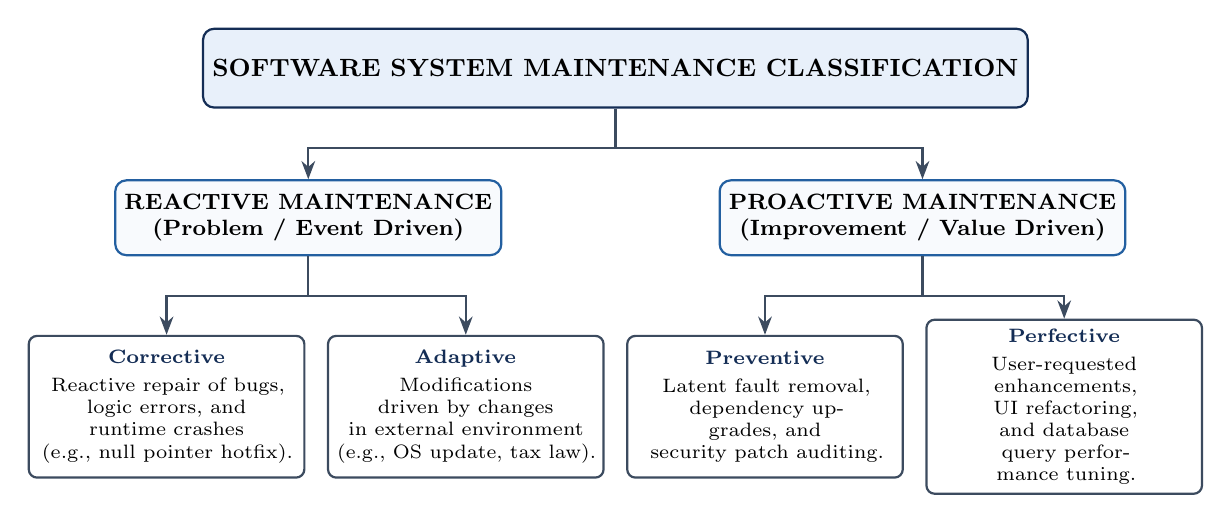
\begin{tikzpicture}[
    root/.style={rectangle, draw=primaryNavy, fill=tableHeader, rounded corners=4pt, minimum width=6.8cm, minimum height=1.0cm, align=center, font=\small\bfseries, thick},
    branch/.style={rectangle, draw=secondaryBlue, fill=lightBg, rounded corners=4pt, minimum width=4.5cm, minimum height=0.95cm, align=center, font=\footnotesize\bfseries, thick},
    leaf/.style={rectangle, draw=slateGray, fill=white, rounded corners=3pt, minimum width=3.5cm, minimum height=1.8cm, text width=3.2cm, align=center, font=\scriptsize, thick},
    arrow/.style={-{Stealth[scale=1.0]}, thick, color=slateGray}
]
    % Root
    \node[root] (top) at (0, 0) {SOFTWARE SYSTEM MAINTENANCE CLASSIFICATION};

    % Branches
    \node[branch] (reactive) at (-3.9, -1.9) {REACTIVE MAINTENANCE\\\footnotesize(Problem / Event Driven)};
    \node[branch] (proactive) at (3.9, -1.9) {PROACTIVE MAINTENANCE\\\footnotesize(Improvement / Value Driven)};

    % Leaves
    \node[leaf] (corrective) at (-5.7, -4.3) {\textbf{\color{primaryNavy}Corrective}\\\vspace{2pt}Reactive repair of bugs,\\logic errors, and runtime crashes\\(e.g., null pointer hotfix).};
    \node[leaf] (adaptive) at (-1.9, -4.3) {\textbf{\color{primaryNavy}Adaptive}\\\vspace{2pt}Modifications driven by changes\\in external environment\\(e.g., OS update, tax law).};

    \node[leaf] (preventive) at (1.9, -4.3) {\textbf{\color{primaryNavy}Preventive}\\\vspace{2pt}Latent fault removal,\\dependency upgrades, and\\security patch auditing.};
    \node[leaf] (perfective) at (5.7, -4.3) {\textbf{\color{primaryNavy}Perfective}\\\vspace{2pt}User-requested enhancements,\\UI refactoring, and database\\query performance tuning.};

    % Links routed cleanly with explicit downward drops
    \draw[arrow] (top.south) -- ++(0,-0.5) -| (reactive.north);
    \draw[arrow] (top.south) -- ++(0,-0.5) -| (proactive.north);

    \draw[arrow] (reactive.south) -- ++(0,-0.5) -| (corrective.north);
    \draw[arrow] (reactive.south) -- ++(0,-0.5) -| (adaptive.north);

    \draw[arrow] (proactive.south) -- ++(0,-0.5) -| (preventive.north);
    \draw[arrow] (proactive.south) -- ++(0,-0.5) -| (perfective.north);
\end{tikzpicture}
\caption{Taxonomy of Software Maintenance: Reactive versus Proactive Engineering Interventions.}
\label{fig:maintenance_taxonomy}
\end{figure}

\begin{conceptcard}{Detailed Exposition of Maintenance Types}
\textbf{1. Corrective Maintenance (Reactive):} The urgent diagnosis, remediation, and patching of documented errors, logic defects, or catastrophic system crashes encountered during operational use. For example, fixing a race condition in a multi-threaded invoice exporter that throws unhandled null pointer exceptions during end-of-month financial closing.

\textbf{2. Adaptive Maintenance (Reactive):} Modifying software to maintain operational compatibility with shifting external environments, including operating systems, hardware platforms, third-party API deprecations, or legal and regulatory mandates. For example, updating an enterprise payroll system to comply with newly enacted tax brackets, or migrating an application from Python~3.8 to Python~3.12 following upstream end-of-life deprecation.

\textbf{3. Preventive Maintenance (Proactive):} Preemptive modifications executed to uncover and remediate latent defects before they manifest as operational outages. This includes refactoring brittle code modules, updating third-party open-source libraries to close newly discovered Common Vulnerabilities and Exposures (CVEs), re-indexing database tables to prevent table scan degradation, and expanding server storage capacity ahead of projected growth.

\textbf{4. Perfective Maintenance (Proactive):} Enhancing software beyond its original functional specifications in response to user feedback or evolving operational needs. This includes redesigning user interface workflows to reduce task completion times, refactoring SQL queries to reduce execution latency, or adding new reporting modules requested by management.
\end{conceptcard}

\subsection{Operational Maintenance Lifecycle Workflow}
Executing maintenance within enterprise environments requires a structured, eight-stage operational workflow to prevent unvetted changes from destabilizing production:

\begin{figure}[htbp]
\centering
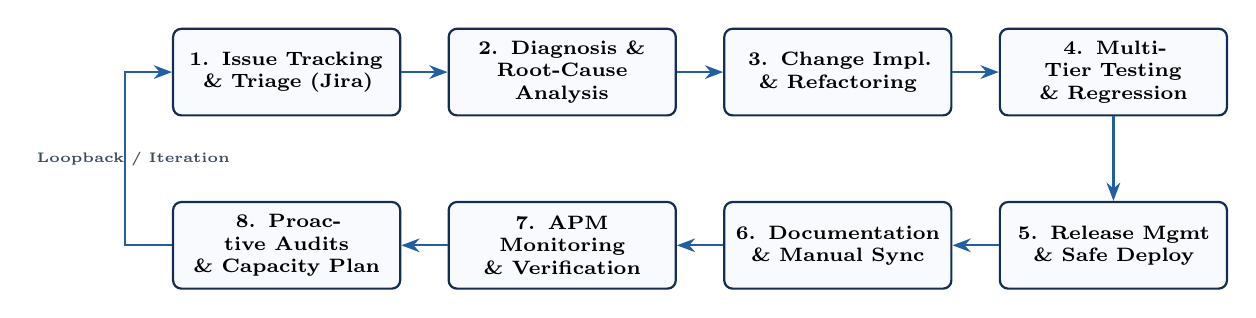
\begin{tikzpicture}[
    stepNode/.style={rectangle, draw=primaryNavy, fill=lightBg, rounded corners=3pt, minimum width=2.85cm, minimum height=1.1cm, text width=2.65cm, align=center, font=\scriptsize\bfseries, thick},
    arrow/.style={-{Stealth[scale=1.0]}, thick, color=secondaryBlue}
]
    % Top Row (1 to 4)
    \node[stepNode] (s1) at (0.0, 3.0) {1. Issue Tracking\\\& Triage (Jira)};
    \node[stepNode] (s2) at (3.5, 3.0) {2. Diagnosis \&\\Root-Cause Analysis};
    \node[stepNode] (s3) at (7.0, 3.0) {3. Change Impl.\\\& Refactoring};
    \node[stepNode] (s4) at (10.5, 3.0) {4. Multi-Tier Testing\\\& Regression};

    % Bottom Row (5 to 8)
    \node[stepNode] (s5) at (10.5, 0.8) {5. Release Mgmt\\\& Safe Deploy};
    \node[stepNode] (s6) at (7.0, 0.8) {6. Documentation\\\& Manual Sync};
    \node[stepNode] (s7) at (3.5, 0.8) {7. APM Monitoring\\\& Verification};
    \node[stepNode] (s8) at (0.0, 0.8) {8. Proactive Audits\\\& Capacity Plan};

    % Connections
    \draw[arrow] (s1) -- (s2);
    \draw[arrow] (s2) -- (s3);
    \draw[arrow] (s3) -- (s4);
    \draw[arrow] (s4) -- (s5);
    \draw[arrow] (s5) -- (s6);
    \draw[arrow] (s6) -- (s7);
    \draw[arrow] (s7) -- (s8);
    \draw[arrow] (s8.west) -- ++(-0.6,0) |- (s1.west);
    \node[left, font=\tiny\bfseries, color=slateGray] at (-0.6, 1.9) {Loopback / Iteration};
\end{tikzpicture}
\caption{The Closed-Loop Eight-Stage Enterprise Maintenance Lifecycle Workflow.}
\label{fig:maintenance_workflow}
\end{figure}

\begin{enumerate}
    \item \textbf{Issue Tracking and Management:} Field incidents, user tickets, or automated APM alerts are ingested into a centralized tracking platform (e.g., Jira, GitHub Issues). Incidents are triaged, assigned severity levels (P1 Critical Blocker to P4 Minor Trivial), and routed to the appropriate engineering teams.
    \item \textbf{Diagnosis and Root-Cause Analysis:} Engineers isolate the precise code block, query, or infrastructure component causing the failure using distributed traces, debuggers, and memory profilers.
    \item \textbf{Change Implementation:} Modifying code, refactoring modules, updating database migrations, and committing changes to branch-isolated version control.
    \item \textbf{Multi-Tier Testing and Regression Verification:} The modified codebase is tested against unit, integration, and full regression suites to confirm the issue is resolved without introducing side-effects.
    \item \textbf{Release Management and Safe Deployment:} The change is packaged and deployed into production using an appropriate deployment pattern (e.g., Canary or Blue-Green) under Change Advisory Board (CAB) supervision.
    \item \textbf{Documentation and Manual Synchronization:} Technical architectural blueprints, API documentation, runbooks, and user training manuals are updated to reflect the modifications.
    \item \textbf{APM Monitoring and Telemetry Verification:} Post-deployment telemetry is monitored in real time using APM dashboards (e.g., Datadog, Prometheus) to verify error reduction and latency stability.
    \item \textbf{Proactive Auditing and Capacity Planning:} Teams review historical incident trends to identify recurring architectural bottlenecks, planning future preventive refactorings.
\end{enumerate}

% =========================================================================
% SECTION 7: IS GOVERNANCE FRAMEWORKS & RISK MANAGEMENT
% =========================================================================
\section[Governance and Risk Management]{Information System Governance Frameworks and Risk Management}
\label{sec:governance}

\subsection{Definition, Purpose, and Strategic Value}
Information System Governance is the overarching framework of leadership, organizational structures, policies, and operational processes that ensure an organization's digital infrastructure sustains and extends its strategic business objectives.

Governance is not mere bureaucratic friction; it is a critical institutional capability that establishes decision-making rights, aligns technical roadmaps with corporate strategy, ensures regulatory compliance, and protects shareholder value from catastrophic operational and security failures.

\subsection{The Four Pillars of IT Governance}
Effective governance relies on four foundational pillars:
\begin{itemize}
    \item \textbf{Policy Development:} Formulating explicit, enforceable organizational standards governing data classifications, access privileges, acceptable technology use, password complexity, and data retention windows.
    \item \textbf{Enterprise Risk Management:} The continuous identification, assessment, quantification, and mitigation of technical, operational, and security risks that could disrupt business operations.
    \item \textbf{Regulatory Compliance Monitoring:} Ensuring the enterprise conforms to applicable regional and international legal mandates, including GDPR, HIPAA, PCI-DSS, and the Sarbanes-Oxley Act (SOX).
    \item \textbf{Change Management and Change Advisory Boards (CAB):} Establishing formal review mechanisms where all proposed production modifications, infrastructure upgrades, and architectural refactorings are evaluated for operational risk, tested for rollback viability, and approved prior to release.
\end{itemize}

\subsection{Comparative Analysis of Standard Governance Frameworks}
To structure their governance programs, modern enterprises implement one or more established international governance frameworks:

\begin{table}[htbp]
\centering
\small
\renewcommand{\arraystretch}{1.25}
\begin{tabularx}{\textwidth}{L{2.4cm} L{3.0cm} L{3.0cm} Y}
\toprule
\rowcolor{tableHeader}
\textbf{Framework} & \textbf{Core Focus Domain} & \textbf{Target Audience} & \textbf{Primary Strategic Benefit} \\
\midrule
\textbf{COBIT} \newline (ISACA) & Comprehensive IT Governance \& Alignment & Enterprise Executives, Board Members, CIOs & Aligns digital strategy with overarching business goals using balanced scorecards and maturity models. \\
\textbf{ITIL} \newline (AXELOS) & IT Service Management (ITSM) Workflows & IT Operations Leads, Service Desk Directors & Standardizes IT service lifecycles (Incident, Problem, Change, and Release Management). \\
\textbf{ISO/IEC 38500} \newline (ISO Standard) & Corporate Governance Principles for IT & Corporate Boards of Directors, C-Suite Leaders & Provides six principles (Responsibility, Strategy, Acquisition, Performance, Conformance, Human Behavior) for IT oversight. \\
\textbf{NIST CSF} \newline (NIST) & Cybersecurity Risk Management & Chief Information Security Officers (CISOs), SecOps & Offers a risk-based cybersecurity structure organized into five functions: Identify, Protect, Detect, Respond, Recover. \\
\bottomrule
\end{tabularx}
\caption{Comprehensive Comparison Matrix of Enterprise Information System Governance Frameworks.}
\label{tab:governance_matrix}
\end{table}

\begin{governancebox}{Core Directives of International Governance Standards}
\textbf{1. COBIT (Control Objectives for Information and Related Technologies):} Published by ISACA, COBIT provides a comprehensive framework bridging the gap between technical teams, business managers, and corporate auditors. It offers metrics, operational scorecards, and maturity models to ensure IT investments deliver business value while managing risk.

\textbf{2. ITIL (Information Technology Infrastructure Library):} The de-facto global standard for IT Service Management (ITSM). ITIL structures IT operations into systematic service lifecycles, establishing formal processes for Service Strategy, Service Design, Service Transition, Service Operation, and Continual Service Improvement.

\textbf{3. ISO/IEC 38500:} An international standard providing corporate boards with guidance on the ethical, legal, and operational oversight of IT. It establishes six core principles: establishing clear responsibilities, planning business strategy, acquiring technology prudently, ensuring adequate performance, confirming legal conformance, and respecting human behavior.

\textbf{4. NIST Cybersecurity Framework (CSF):} Developed by the U.S. National Institute of Standards and Technology, this framework provides a prioritized, flexible approach to managing cybersecurity risk. It is organized around five core functions: \textbf{Identify} assets and risks, \textbf{Protect} critical infrastructure with access controls, \textbf{Detect} security anomalies, \textbf{Respond} effectively to incidents, and \textbf{Recover} operational capabilities post-breach.
\end{governancebox}

% =========================================================================
% SECTION 8: IS SECURITY, CYBER THREATS, & DEFENSIVE SAFEGUARDS
% =========================================================================
\section[Information System Security]{Information System Security, Cyber Threats, and Safeguards}
\label{sec:security}

\subsection{Core Security Principles: The CIA Triad}
Information System Security encompasses all technological, physical, and procedural controls designed to safeguard an organization's digital assets from unauthorized access, disruption, modification, or destruction. System security is founded upon the classical benchmark model known as the \textbf{CIA Triad}:

\begin{figure}[htbp]
\centering
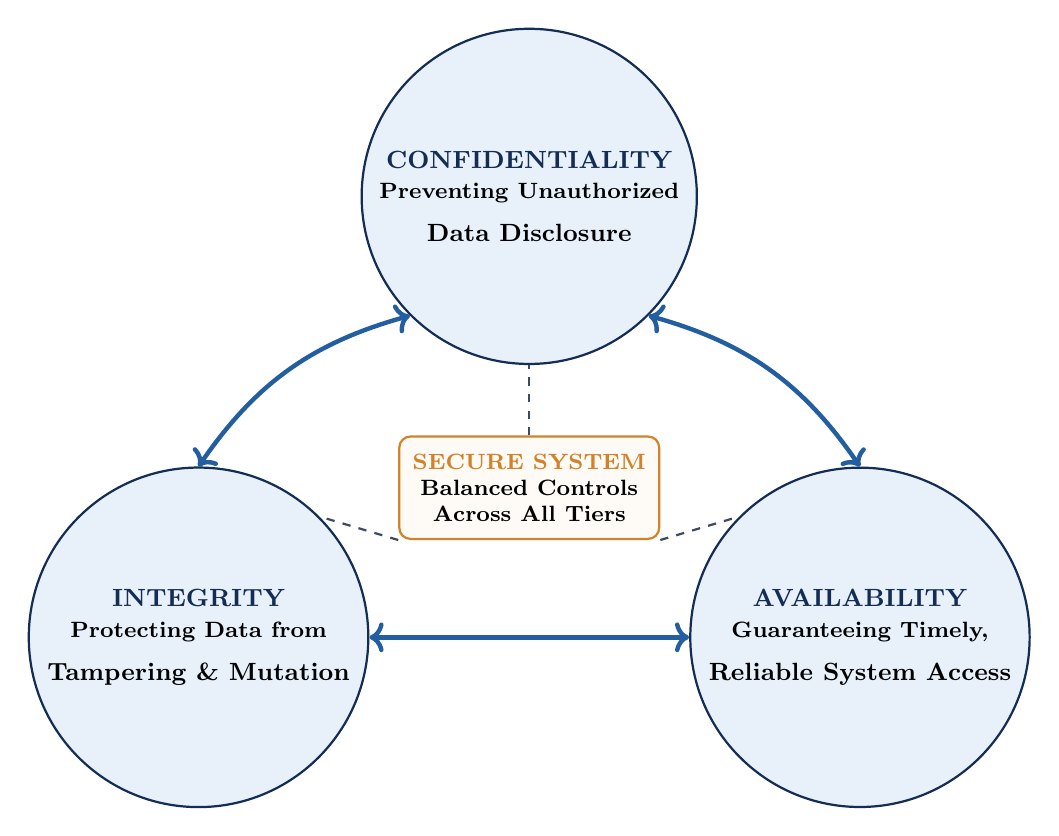
\begin{tikzpicture}[
    triad/.style={circle, draw=primaryNavy, fill=tableHeader, minimum size=3.3cm, align=center, font=\small\bfseries, thick},
    centerBox/.style={rectangle, draw=caseBorder, fill=caseBg, rounded corners=4pt, minimum width=3.3cm, minimum height=1.3cm, align=center, font=\footnotesize\bfseries, thick}
]
    % Triad Nodes in Equilateral Geometry
    \node[triad] (conf) at (0, 3.8) {\textbf{\color{primaryNavy}CONFIDENTIALITY}\\\vspace{3pt}\footnotesize Preventing Unauthorized\\Data Disclosure};
    \node[triad] (integ) at (-4.2, -1.8) {\textbf{\color{primaryNavy}INTEGRITY}\\\vspace{3pt}\footnotesize Protecting Data from\\Tampering \& Mutation};
    \node[triad] (avail) at (4.2, -1.8) {\textbf{\color{primaryNavy}AVAILABILITY}\\\vspace{3pt}\footnotesize Guaranteeing Timely,\\Reliable System Access};

    % Center Node
    \node[centerBox] (core) at (0, 0.1) {\textbf{\color{caseBorder}SECURE SYSTEM}\\Balanced Controls\\Across All Tiers};

    % Perimeter Connectors (curved outside the center node)
    \draw[<->, ultra thick, color=secondaryBlue] (conf.south west) to[bend right=20] (integ.north);
    \draw[<->, ultra thick, color=secondaryBlue] (integ.east) -- (avail.west);
    \draw[<->, ultra thick, color=secondaryBlue] (avail.north) to[bend right=20] (conf.south east);

    % Radial Spokes from Core
    \draw[dashed, thick, color=slateGray] (core.north) -- (conf.south);
    \draw[dashed, thick, color=slateGray] (core.south west) -- (integ.north east);
    \draw[dashed, thick, color=slateGray] (core.south east) -- (avail.north west);
\end{tikzpicture}
\caption{The Classical CIA Security Triad and Balanced System Protection.}
\label{fig:cia_triad}
\end{figure}

\begin{itemize}
    \item \textbf{Confidentiality:} Ensuring that sensitive, proprietary, or personal information is accessible only to authorized entities, processes, and systems. Confidentiality controls include cryptographic encryption, access control lists (ACLs), multi-factor authentication, and data classification.
    \item \textbf{Integrity:} Safeguarding the accuracy, completeness, and authenticity of data and software logic against unauthorized modification, tampering, or malicious corruption. Integrity controls include cryptographic hash checksums (e.g., SHA-256), digital signatures, database transaction constraints, and write-once-read-many (WORM) audit logs.
    \item \textbf{Availability:} Ensuring that systems, communication networks, and data repositories remain consistently operational and accessible to authorized users when needed. Availability controls include redundant power supplies, multi-zone server failover, distributed load balancers, DDoS mitigation scrubbers, and rapid disaster recovery pipelines.
\end{itemize}

\subsection{The Four Technical Security Pillars}
Operationalizing security across an enterprise software system requires four core technical controls:
\begin{enumerate}
    \item \textbf{Authentication Mechanisms:} The cryptographic and procedural verification of an entity's claimed identity. Modern standards demand Multi-Factor Authentication (MFA), combining something the user knows (passwords, passphrases), something the user has (hardware FIDO2 security keys, TOTP authenticator tokens), and something the user is (biometric fingerprint or facial scans).
    \item \textbf{Access Control and Authorization:} The enforcement of fine-grained permissions once identity is established. Enterprise architectures rely primarily on \textbf{Role-Based Access Control (RBAC)}, where permissions are mapped to organizational roles, and \textbf{Attribute-Based Access Control (ABAC)}, which evaluates context (user role, network IP, time of access, device posture) under a Zero-Trust architecture.
    \item \textbf{Cryptographic Encryption:} Protecting information assets throughout their lifecycle:
    \begin{itemize}
        \item \textit{Data-in-Transit:} Encrypting network streams using TLS 1.3 to prevent eavesdropping and man-in-the-middle (MitM) packet inspection.
        \item \textit{Data-at-Rest:} Encrypting databases, file storage volumes, and backup media using AES-256 with hardware security module (HSM) key management.
    \end{itemize}
    \item \textbf{Incident Management and Disaster Recovery:} The predefined procedures for detecting, containing, investigating, and recovering from security breaches. This encompasses Computer Security Incident Response Teams (CSIRT), Security Information and Event Management (SIEM) log aggregators, and off-site immutable backup restoration.
\end{enumerate}

\subsection{Cyber Threat Landscape and Proactive Defensive Controls}
Organizations face an evolving cyber threat landscape, including polymorphic malware, ransomware that encrypts corporate databases, spear-phishing attacks targeting employee credentials, Distributed Denial of Service (DDoS) botnets that flood application gateways, and insider threats exploiting privileged access.

To counter these threats, software engineering teams must implement four core defensive controls:
\begin{itemize}
    \item \textbf{Automated Patch Management:} The rapid deployment of vendor security patches across operating systems, runtime libraries, and third-party dependencies within strict change-management windows.
    \item \textbf{Immutable, Air-Gapped Data Backups:} Maintaining offline, cryptographically isolated, write-once backups that cannot be encrypted or deleted by ransomware actors during an active breach.
    \item \textbf{Continuous Employee Security Awareness Training:} Educating staff to identify social engineering schemes, spear-phishing attempts, and credential-harvesting attacks.
    \item \textbf{Rigorous Penetration Testing:} Engaging certified ethical hackers to conduct adversarial penetration testing and vulnerability assessments, discovering attack vectors before malicious actors exploit them.
\end{itemize}

% =========================================================================
% SECTION 9: ETHICS, DATA PRIVACY, & ALGORITHMIC GOVERNANCE
% =========================================================================
\section[Ethics and Algorithmic Governance]{Ethics, Data Privacy, and Algorithmic Governance}
\label{sec:ethics}

\subsection{Foundations of Ethics in Information Systems}
Information Systems Ethics examines the moral obligations, human rights considerations, and societal impacts inherent in the design, development, and operation of digital technologies. As software systems increasingly automate critical decisions in healthcare, financial lending, employment, and public administration, software engineers hold significant societal responsibility. Writing code is not merely a technical exercise; it directly affects human dignity, personal liberty, and economic opportunity.

\subsection{The Four Core Ethical Principles}
Ethical system analysis and design is guided by four foundational principles:
\begin{itemize}
    \item \textbf{Privacy:} Respecting personal autonomy by treating an individual's Personally Identifiable Information (PII) as private by default. Systems must collect only the minimum data necessary for a stated transaction and delete it once the purpose is served.
    \item \textbf{Transparency:} Providing users with clear, accessible visibility into how their data is collected, processed, and monetized, as well as explaining how automated decision models derive their conclusions.
    \item \textbf{Accountability:} Establishing legal, organizational, and moral responsibility for system errors, algorithmic harms, or security failures, ensuring that organizations cannot hide behind automated processes.
    \item \textbf{Fairness:} Guaranteeing that digital services and algorithmic models treat individuals equitably, without unlawful bias based on race, gender, socio-economic status, or geographic origin.
\end{itemize}

\subsection{Systemic Ethical Dilemmas in Digital Technologies}
Modern information systems confront four major ethical dilemmas:
\begin{enumerate}
    \item \textbf{Covert Data Harvesting and User Monetization:} Commercial software that collects detailed user activity, location coordinates, and biometric data without meaningful consent, monetizing it through third-party data brokers and behavioral advertising networks.
    \item \textbf{Algorithmic Bias and Machine Discrimination:} Machine learning models trained on historical data often absorb and amplify societal prejudices. Examples include automated resume-screening algorithms that downgrade female candidates, or automated credit-scoring models that penalize marginalized communities.
    \item \textbf{Invasive Surveillance and Behavioral Manipulation:} The deployment of invasive telemetry, workplace monitoring tools, and social media feed algorithms that exploit cognitive vulnerabilities to drive addictive engagement, degrade mental health, and polarize public discourse.
    \item \textbf{The Digital Divide:} System designs that assume ubiquitous high-speed broadband and high-end hardware, inadvertently excluding low-income and rural populations from accessing essential digital government and banking services.
\end{enumerate}

\subsection{Proactive Ethical Engineering Safeguards}
To prevent ethical failures, software engineering teams must institutionalize proactive engineering safeguards:
\begin{itemize}
    \item \textbf{Independent Algorithmic Audits:} Subjecting predictive algorithms and automated decision models to rigorous statistical audits (e.g., assessing demographic parity and equal opportunity metrics) to detect and correct algorithmic bias before public release.
    \item \textbf{Universal Accessibility Standards (WCAG):} Designing digital user interfaces that comply with the Web Content Accessibility Guidelines (WCAG 2.1 AA/AAA), ensuring equitable usability for individuals with visual, auditory, motor, or cognitive impairments.
    \item \textbf{Plain-Language Consent and Transparency Disclosures:} Replacing dense, confusing legal agreements with straightforward, layered consent dialogs that inform users about data handling in clear language.
\end{itemize}

% =========================================================================
% SECTION 10: APPLIED CASE STUDIES & PRACTICAL ACTIVITIES
% =========================================================================
\section[Applied Case Studies]{Applied Case Studies and Problem-Solving Activities}
\label{sec:case_studies}

To demonstrate how the theoretical principles of testing, deployment, maintenance, governance, and ethics apply to real-world software engineering, this section presents four applied case studies adapted from the curriculum.

\subsection{Case Study 1: Mobile App Integration Failure}
\begin{casestudybox}{Mobile Application Authentication and Cloud Synchronization Failure}
\textbf{The Operational Scenario:} A cross-platform mobile application featuring user registration, cloud database synchronization, and push notifications launches in production. Immediately following launch, customer support is flooded with complaints: newly registered users are unable to synchronize their local application data with the cloud server, receiving continuous ``Sync Failed'' errors. However, existing users who registered during previous beta cycles experience no synchronization issues.

\textbf{Diagnostic Root-Cause Analysis:}
\begin{enumerate}
    \item \textit{Interface Parameter Passing Failure:} The local registration module authenticates new user accounts successfully on the local device, but fails to pass the newly generated cryptographic session bearer token to the background cloud synchronization worker thread.
    \item \textit{Distributed Database Race Condition:} An asynchronous race condition exists in the registration workflow. The mobile client initiates data synchronization before the cloud backend commits the new user's database record. Consequently, the cloud sync worker queries for a non-existent account ID, triggering an unhandled database Foreign Key rejection.
\end{enumerate}

\textbf{Remediation and Integration Test Plan:}
\begin{itemize}
    \item \textit{Test Case 1 (Token Propagation):} Construct an automated integration test verifying that upon the execution of the registration callback, a valid JWT bearer token is received, decoded, and injected into the background sync client's authentication headers.
    \item \textit{Test Case 2 (Asynchronous Handshake Verification):} Refactor the client-side architecture to await an explicit HTTP 201 Created confirmation and database lock release from the cloud API prior to scheduling the initial sync job.
    \item \textit{Test Case 3 (Negative Token Rejection):} Verify that when an expired or malformed token is passed, the sync client catches the HTTP 401 error gracefully, halts sync retries, and prompts the user to re-authenticate without corrupting local data.
\end{itemize}
\end{casestudybox}

\subsection{Case Study 2: Healthcare System Blue-Green Deployment}
\begin{casestudybox}{Zero-Downtime Deployment and Database State Synchronization}
\textbf{The Operational Scenario:} An enterprise hospital information platform that manages patient medical records, bed allocations, and prescription dispensing prepares to deploy a major software release (v2.0). Because the hospital operates 24/7/365, scheduled maintenance downtime is prohibited. The engineering team adopts a Blue-Green deployment model. While application server traffic shifts smoothly at the router level, concerns emerge regarding database state consistency between the Blue (v1.0) and Green (v2.0) environments during the transition window.

\textbf{Resolution and Data Integrity Strategy:}
\begin{enumerate}
    \item \textit{Backward-Compatible Schema Migration (Expand-Contract Pattern):} Database schema modifications are decoupled from application releases. The database schema is first ``expanded'' with nullable or default-valued fields that support both v1.0 and v2.0 queries concurrently, ensuring neither version encounters syntax exceptions.
    \item \textit{Synchronous Dual-Writing / Read-Replication:} During the transition window, write transactions are replicated across both database clusters using synchronous two-phase commits, guaranteeing that transactions committed by doctors on Blue are reflected in Green.
    \item \textit{Brief Read-Only Lock Window for Final Cutover:} At the precise moment of DNS cutover, the Blue environment is placed in a brief read-only maintenance mode (lasting less than 3 seconds), ensuring all pending transactions drain into the database before the router directs write traffic to Green.
\end{enumerate}
\end{casestudybox}

\subsection{Case Study 3: Enterprise Analytical Report Export Out-Of-Memory Crash}
\begin{casestudybox}{Corrective Maintenance for Analytical Out-Of-Memory Outages}
\textbf{The Operational Scenario:} Corporate finance users report that an enterprise ERP application repeatedly crashes whenever they attempt to export comprehensive end-of-quarter financial audits to Excel or PDF. During the export process, the entire application server becomes unresponsive, dropping active sessions for all connected users and forcing an emergency server restart.

\textbf{Operational Maintenance Workflow and Remediation:}
\begin{enumerate}
    \item \textit{Classification:} \textbf{Corrective Maintenance} (urgent repair of an operational crash).
    \item \textit{Issue Tracking (Jira):} A critical P1 ticket is created, attaching server system error logs and memory heap dumps.
    \item \textit{Diagnosis and Profiling:} Memory heap inspection using Eclipse Memory Analyzer (MAT) reveals a \texttt{java.lang.OutOfMemoryError: Java heap space}. The reporting module executes an unpaginated SQL query that loads over 850,000 dense financial rows into memory simultaneously, exhausting the 8GB server heap.
    \item \textit{Code Refactoring and Remediation:} Engineers refactor the data exporter to use streaming database cursors and chunked batch pagination (processing 1,000 records at a time) and stream the output directly to the HTTP response socket, keeping memory consumption under 50MB.
    \item \textit{Testing and Verification:} The refactored code is subjected to staging load tests using a 1,000,000-row synthetic dataset to confirm memory stability under sustained concurrent exports.
    \item \textit{Release and APM Tracking:} Deployed via a rolling update; server heap usage is tracked continuously using Datadog APM dashboards to ensure long-term stability.
\end{enumerate}
\end{casestudybox}

\subsection{Case Study 4: Covert User Activity Harvesting for Ad Networks}
\begin{casestudybox}{Ethical Violation and Data Privacy Remediation}
\textbf{The Operational Scenario:} A commercial mobile software vendor quietly incorporates third-party telemetry SDKs into its consumer utility application. The software silently captures user location trails, contact lists, and device usage logs in the background, transmitting the unencrypted data to third-party advertising brokers for behavioral monetization without explicit user consent.

\textbf{Ethical and Regulatory Evaluation:}
\begin{itemize}
    \item \textit{Violations of Ethical Foundations:} Direct breach of \textbf{Privacy} (non-consensual harvesting of personal data), \textbf{Transparency} (concealing data monetization practices from users), and \textbf{Accountability} (violating consumer trust and failing fiduciary duties).
    \item \textit{Legal and Regulatory Exposure:} Severe non-compliance with the General Data Protection Regulation (GDPR Article~6 on lawful processing) and the California Consumer Privacy Act (CCPA), exposing the company to major regulatory penalties.
\end{itemize}

\textbf{Actionable Engineering Remediation Plan:}
\begin{enumerate}
    \item \textit{Implementation of Explicit Opt-In Modals:} Redesign application onboarding to introduce clear, unbundled opt-in consent dialogs before collecting any non-essential telemetry.
    \item \textit{Data Minimization Architecture:} Purge all non-essential telemetry tracking code. Enforce automated data retention policies that delete or anonymize collected logs after 30 days.
    \item \textit{Transparent Disclosures:} Publish an accessible, plain-language Privacy Policy detailing all data handling practices and providing users with self-service data deletion controls.
\end{enumerate}
\end{casestudybox}

% =========================================================================
% SECTION 11: TECHNICAL GLOSSARY
% =========================================================================
\section[Technical Glossary]{Comprehensive Technical Glossary}
\label{sec:glossary}

To support undergraduate revision and serve as a reliable reference, this glossary defines the key technical terms from Lectures~9 and~10:

\begin{description}[leftmargin=!,labelwidth=4.5cm]
    \item[Acceptance Testing] The final formal stage of testing, conducted to verify whether an integrated application satisfies all business specifications required for formal client sign-off.
    \item[Adaptive Maintenance] System modifications executed to ensure continued compatibility with changing technical, operating system, hardware, or regulatory environments.
    \item[Algorithmic Bias] Systematic, repeatable errors in computer algorithms that generate unfair outcomes, favoring or penalizing arbitrary demographics.
    \item[API (Application Programming Interface)] A formal specification of software interfaces, parameter signatures, and communication protocols enabling distinct applications to exchange data.
    \item[Blue-Green Deployment] A zero-downtime release methodology utilizing two identical production environments (Blue and Green) where live traffic is switched at the router level.
    \item[Bug] An internal runtime flaw, fault, or aberrant code state within an executable software program resulting from an underlying human error.
    \item[Canary Deployment] A deployment pattern where an update is exposed to a tiny fraction of live users (e.g., 5\%) to validate system metrics before full-scale rollout.
    \item[CIA Triad] Confidentiality, Integrity, and Availability---the foundational benchmark model governing information system security engineering.
    \item[COBIT] Control Objectives for Information and Related Technologies---an international IT governance framework aligning digital strategy with business goals.
    \item[Corrective Maintenance] Reactive technical modifications executed to diagnose and repair software bugs, logic flaws, or system crashes occurring in production.
    \item[Defect] A formal, documented variance between the observed runtime behavior of a software system and its required specification.
    \item[Driver] A specialized test harness code module used in bottom-up integration testing to simulate higher-level calling routines.
    \item[Encryption] The cryptographic transformation of plaintext data into unreadable ciphertext using mathematical algorithms (e.g., AES-256) to prevent unauthorized inspection.
    \item[Error] A cognitive mistake, conceptual misunderstanding, or syntax error made by a software engineer, systems analyst, or designer.
    \item[Feature Toggle] A software engineering pattern enabling or disabling functionality dynamically at runtime without redeploying code.
    \item[Integration Testing] The systematic evaluation of data exchanges, interface contracts, and communication protocols among integrated software modules.
    \item[ITIL] Information Technology Infrastructure Library---a comprehensive framework establishing best practices for IT Service Management (ITSM).
    \item[Perfective Maintenance] Proactive software modifications executed to improve system performance, maintainability, or user experience based on operational feedback.
    \item[Preventive Maintenance] Proactive engineering interventions designed to eliminate latent defects and security vulnerabilities before they cause outages.
    \item[Regression Testing] Re-executing test suites following code modifications to confirm that bug fixes or refactoring have not degraded existing functions.
    \item[Shadow Deployment] A release pattern where incoming live production traffic is mirrored asynchronously to a new version fleet in the background with zero user impact.
    \item[Stub] A dummy code module used in top-down integration testing to simulate unbuilt lower-level subroutines by returning hardcoded test responses.
    \item[System Testing] End-to-end evaluation of a fully integrated software application against its documented system requirements.
    \item[Unit Testing] The isolated verification of individual methods, subroutines, or classes in complete independence from external dependencies.
\end{description}

% =========================================================================
% SECTION 12: ACADEMIC REFERENCES & BIBLIOGRAPHY
% =========================================================================
\section[References and Bibliography]{Academic References and Bibliography}
\label{sec:references}

The principles, methodologies, and frameworks synthesized in this treatise are grounded in the core literature of software engineering and information systems analysis:

\begin{enumerate}[label={[\arabic*]}]
    \item Pressman, R.~S. (2010). \textit{Software Engineering: A Practitioner's Approach} (7th ed.). McGraw-Hill Education. [Cited in Lecture~9, Slide~60; Lecture~10, Slide~25].
    \item Senn, J.~A. (2000). \textit{Analysis and Design of Information Systems} (2nd ed.). Tata McGraw-Hill Education. [Cited in Lecture~9, Slide~62; Lecture~10, Slide~26].
    \item Awad, E.~M. (2000). \textit{System Analysis and Design} (2nd ed.). Galgotia Publications. [Cited in Lecture~9, Slide~62; Lecture~10, Slide~26].
    \item Dennis, A., Wixom, B.~H., \& Roth, R.~M. (2012). \textit{Systems Analysis and Design} (5th ed.). John Wiley \& Sons, Inc. [Cited in Lecture~9, Slide~62; Lecture~10, Slide~26].
    \item Rajaraman, V. (2000). \textit{Analysis and Design of Information Systems}. PHI Learning Pvt. Ltd. [Cited in Lecture~9, Slide~62; Lecture~10, Slide~26].
    \item Kelly, J.~C., Sherif, J.~S., \& Hops, J. (1992). An analysis of defect densities found during software inspections. \textit{Journal of Systems and Software}, 17(2), 111--117. [Cited in Lecture~9, Slide~61; Lecture~10, Slide~25].
    \item Bhandari, I., Halliday, M.~J., Chaar, J., Chillarege, R., Jones, K., Atkinson, J.~S., \& Yonezawa, M. (1994). In-process improvement through defect data interpretation. \textit{IBM Systems Journal}, 33(1), 182--214. [Cited in Lecture~9, Slide~61; Lecture~10, Slide~25].
    \item Sardar, M.~S. (2000). \textit{System Analysis and Design}. Shri Gavisiddheshwara Arts, Science \& Commerce College. [Cited in Lecture~9, Slide~61; Lecture~10, Slide~26].
    \item Ayepeku, F.~O. (n.d.). \textit{System Analysis and Design Lecture Notes} (CSC 308). Mathematical and Computing Science Department. [Cited in Lecture~9, Slide~62; Lecture~10, Slide~27].
    \item Nwaocha, V. (2009). \textit{Advanced Systems Analysis and Design}. National Open University of Nigeria. [Cited in Lecture~9, Slide~63; Lecture~10, Slide~27].
\end{enumerate}

\end{document}

